%% 
%% ACS project dissertation template. 
%% 
%% Currently designed for printing two-sided, but if you prefer to 
%% print single-sided just remove ",twoside,openright" from the 
%% \documentclass[] line below. 
%%
%%
%%   SMH, May 2010. 

\documentclass[a4paper,12pt]{report}
%TC:group tabular 1 1


%%
%% EDIT THE BELOW TO CUSTOMIZE
%%

\def\authorname{Xiu Hong\ Kooi\xspace}
\def\authorcollege{Wolfson College\xspace}
\def\authoremail{xhk20@cam.ac.uk}
\def\dissertationtitle{Refinement Types in Real-World Programming}
\def\wordcount{0}


%\usepackage[dvips]{epsfig,graphics} 
\usepackage{epsfig,graphicx,verbatim,parskip,tabularx,setspace,xspace}
\usepackage{amsfonts}
\usepackage{amsmath}
\usepackage{amssymb}
\usepackage{listings}
\usepackage{semantic}
\usepackage{float}
\usepackage[margin=3cm]{geometry}


\usepackage{tabto}

\newenvironment{tabs}[1]
 {\flushleft\TabPositions{#1}}
 {\endflushleft}

\usepackage[british]{babel}
\usepackage[%
  backend=bibtex      % biber or bibtex
%,style=authoryear    % Alphabeticalsch
 ,style=numeric-comp  % numerical-compressed
 ,sorting=anyt        % no sorting
 ,sortcites=true      % some other example options ...
 ,maxbibnames=99
 ,block=none
 ,indexing=false
 ,citereset=none
 ,isbn=true
 ,url=true
 ,doi=true            % prints doi
 ,natbib=true         % if you need natbib functions
]{biblatex}
\usepackage{biblatex}
\addbibresource{./dissertation.bib}


%% START OF DOCUMENT
\begin{document}


%% FRONTMATTER (TITLE PAGE, DECLARATION, ABSTRACT, ETC) 
\pagestyle{empty}
\singlespacing
% title page information
\begin{titlepage} 

\begin{center}
\noindent
\huge
\dissertationtitle \\
\vspace*{\stretch{1}}
\end{center}

\begin{center}
\noindent
\huge
\authorname \\
\Large
\authorcollege      \\[24pt]
\mbox{}\\
%\begin{figure}
\includegraphics{CUni3.pdf}
%\end{figure}
\end{center}

\vspace{24pt} 

\begin{center}
\noindent
\large
{\it A dissertation submitted to the University of Cambridge \\ 
in partial fulfilment of the requirements for the degree of \\ 
Master of Philosophy in Advanced Computer Science} 
\vspace*{\stretch{1}}
\end{center}

\begin{center}
\noindent
University of Cambridge \\
Computer Laboratory     \\
William Gates Building  \\
15 JJ Thomson Avenue    \\
Cambridge CB3 0FD       \\
{\sc United Kingdom}    \\
\end{center}

\begin{center}
\noindent
Email: \authoremail \\
\end{center}

\begin{center}
\noindent
\today
\end{center}

\end{titlepage} 

\newpage
\vspace*{\fill}

\onehalfspacing
\newpage
{\Huge \bf Declaration}

\vspace{24pt} 

I \authorname of \authorcollege, being a candidate for the M.Phil in
Advanced Computer Science, hereby declare that this report and the
work described in it are my own work, unaided except as may be
specified below, and that the report does not contain material that
has already been used to any substantial extent for a comparable
purpose.

\vspace{24pt}
Total word count: \wordcount

\vspace{60pt}
\textbf{Signed}: 

\vspace{12pt}
\textbf{Date}:


\vfill

This dissertation is copyright \copyright 2020 \authorname. 
\\
All trademarks used in this dissertation are hereby acknowledged.



\newpage
\vspace*{\fill}

\singlespacing
\newpage
{\Huge \bf Acknowledgement}
\vspace{24pt} 


Write an acknowledgment


\newpage
\vspace*{\fill}

\singlespacing
\newpage
{\Huge \bf Abstract}
\vspace{24pt} 


Write a summary of the whole thing. Make 
sure it fits in one page. 


\newpage
\vspace*{\fill}


\pagenumbering{roman}
\setcounter{page}{0}
\pagestyle{plain}
\tableofcontents
\listoffigures

\onehalfspacing

%% START OF MAIN TEXT 

\chapter{Introduction}
\pagenumbering{arabic} 
\setcounter{page}{1} 

\textit{Type systems} \cite{typesystem} have been one of the most extensively researched field in 
Programming Languages. They act as a way of improving the reliability of a 
language by enforcing rules, preventing operations being applied on 
incompatible data. Type systems can be broken down into various categories but 
two of the most well known are \textit{Static} \cite{staticTyping} and 
\textit{Dynamic} \cite{dynamicTyping} typing. Mainstream programming 
languages such as \textit{Java} \cite{java}, \textit{C} \cite{c} and \textit{C++} \cite{cpp} 
uses the former while languages like \textit{Python} \cite{python} and 
\textit{JavaScript} \cite{js} use the latter. 
Over the years, programming languages have included more powerful and flexible 
type systems, languages like \textit{C\#} \cite{cSharp} and \textit{Go} 
\cite{goInferenceType} allow \textit{type inference} \cite{inferenceType}.

\par
Types are a fundamental way of showing a program's correctness, the use of types 
restricts and therefore eliminates illegal programs at compile time. However, 
even a well-typed program still leaves room for various errors such as 
\begin{enumerate}
  \item {\textbf{Out of bounds access}} In the case of arrays or buffers, the type checker 
  can guarantee that the programmer is using an integer to index elements. 
  However it makes no guarantee that the index is indeed within the valid range. 
  \item {\textbf{Arithmetic errors}} An arithmetic operation can type check that it is 
  indeed operating on numerical values however it is unable to verify the 
  legality. Forbidden arithmetic operations such as as zero divisors or square 
  root of a negative number cannot be type checked. 
  \item {\textbf{Logical error}} Finally, a type checker cannot verify any logical 
  mistakes made by the programmer. Mistakes are inevitable, while the programmer 
  can ensures that the arguments passed to a function are two integers, there is 
  no way for the type checker to ensure that the result is the sum of the two. 
\end{enumerate}

\par
\textit{Dependent Types} \cite{depenTypeAtWork} appears to be a potential solution 
to the problem, dependent types allow the programmer to create types whose 
definition depends on values, e.g. a type of vector that is length $n$. 
A type system that provides such refined control over the values it 
can take unlocks possibility that are previously unavailable such as 
domain-specific type checking.

\par
A slight restriction on dependent types can be found in \textit{Refinement 
Types} \cite{refinementTypes} where one is allowed to define specify subtypes 
of existing types, e.g. a type of non-zero integers. 
A refinement types is constrained by a decidable predicate, 
bringing a better ease of programming. While dependent types are significantly 
more powerful than refinement types, the latter provides a good balance between 
expressiveness and ease of use.

\section{Overview of Refinement Types}
In this section we will discuss at a very high level the behaviour one would 
expect from refinement types and the benefits of using refinement types. 

\begin{figure}[h] 
  \begin{lstlisting}[mathescape=true] 
  type EvenInt = {v : int | v % 2 == 0}
  
  function f(int x) {
    if (x % 2 != 0) 
      throw error ``x has to be even''
    ...
  }
  
  function refined_f(EvenInt i) {
    ...
  }
  \end{lstlisting}
  \caption{Example of Refinement Types}
  \label{code:refine}
\end{figure}

\par
Consider the pseudo-code in figure \ref{code:refine} and assume that the function 
\textit{f} is an arbitrary function that requires the argument $x$ to be even.
The implementation first checks if the value provided is indeed even, if it 
is not then it throws a runtime error. Alternative, the function \textit{refined\_f} 
achieves the same through the use of refinement types. \textit{EvenInt} is a 
integer type whose value is guaranteed to be even. If one passes an odd integer 
to the function it will be caught automatically either at compile time or 
runtime. 

\par
Refinement types allows programmer to define much richer and expressive types 
which can be type checked at run time if not compile time. The addition 
of refinement types allows for safer code as it is able to guarantee certain 
properties. Furthermore, using refinement types eliminates the need for many 
trivial error handling code. Around 4\% of code in every program is 
dedicated to error handling \cite{errorHandlingCode}, refinement types 
can reduce the numbers of checks needed and allow the programmer more time to 
focus on writing the logical part of the code, indirectly 
leading to more robust codebases \cite{elimArrayCheck}.

\section{Motivation}
Type systems have been studied extensively, however dependent and refinement types 
are uncommon in real-world programming. While their theory has been 
established several decades ago, only a small number of programming languages 
support these advanced type systems. Furthermore, the languages that do support 
them are limited to functional languages and theorem provers that are rarely 
used in real-world programming.

\par
The expressive nature of dependent types and refinement types allow one to 
define complex mathematical assertions and hence lends itself to 
theorem proving systems. Multiple functional languages such as \textit{Epigram} 
\cite{epigram} and \textit{Agda} \cite{agda} have 
built in support for dependent typing. However 
mainstream languages such as Java and C++ do not get the luxury.

\par
We note that one of the challenges of adopting dependent and refinement types 
in an imperative programming languages is the presence of mutation. Imperative 
languages rely on statements that change the state of the program, these 
changes has the potential making the semantics of refinement types unclear. 
For instance, if one defined a refinement type as 
$\{\upsilon : int\text{ }|\text{ }\upsilon < N\}$, what is the 
behaviour if the value of $N$ changes?

\par
Past research has studied and shown the feasibility of a dependently typed 
imperative language, however these studies that are focused on expressing 
the semantics of dependent types in an imperative language are often highly 
technical and complex, requiring prerequisite knowledge in the literature. While 
we find these works novel and made important advancements in the field, 
they fail to capture how these types systems could relate to 
mainstream programming languages.

\par
We argue that the the research in the area of dependent types and refinement 
types can be made more accessible. Research in the area often assumes full 
knowledge of \textit{The Lambda Calculus} \cite{lambdaCalculus} and uses 
the concept of \textit{Monads} \cite{monads} for state changes. The semantics 
of the $\lambda$-calculus is simple and naturally 
relates to functional programming languages, however, when one tries to model 
imperative programming by extending the calculus, we begin to lose the simple 
nature. 

\par
Our project is motivated by the apparent lack of accessible literature on the 
theory of refinement types especially involving mainstream languages 
with features such as mutation. We aim to present a simple, restricted framework that 
captures the essence of refinement types. The said framework will be presented as 
an extension to \textit{WHILE language} \cite{whileLanguage}. The WHILE language was 
created as a tool to aid the study of programming language theory, 
thus we believe it strongly satisfies our requirement of accessibility with 
its simple syntax and semantics. Using the 
framework, we will study the interactions between mutation and refinement types 
and relate our findings to concepts in mainstream languages. We believe that 
imperative languages proves to be the more popular paradigm in modern 
programming and is more accessible to the majority. 


\section{Key Contributions}
At the end of the project we achieved the following, 
\begin{enumerate}
  \item Survey the state of dependent and refinement types in 
  real-world programming languages and analyse their differences.
  \item Construct Simple-$R$, an imperative language with refinement types 
  based on the WHILE language resembling C. 
  \item Explore the ambiguity of refinement types in a mutable environment 
  and propose a solution to resolve the ambiguity.
  \item Discuss how the strategies used to handle refinement types in 
  Simple-$R$ are closely tied to concepts in real-world languages.  
  \item Discuss how our work complements the existing literature and possible 
  future extensions.
\end{enumerate}

\par
This dissertation serves as a document for our findings and is organised as 
follows. This first chapter outlines our motivation for this project and our 
contributions. 

\par
In chapter \ref{chapter:background} we provide a background of the area, we 
first give the formal definition of dependent types and how it differs 
from refinement types. We then survey the current state of 
dependent types and refinement types in existing programming languages. 
We explore different languages with varying paradigms and summarise their 
differences in order to have a better understanding of how they 
support these advanced type systems. The languages that are studied include 
Agda, Haskell, Idris, Scala, TypeScript and Xanadu. Finally, we studied 
C++ and how one can construct a limited form of refinement type using the 
template mechanism. 

\par
In chapter \ref{chapter:key_concepts} we identify several key concepts in 
programming language that are relevant to our project. We explain 
and show examples of these concepts in action. Some mechanics are in programming 
languages are non-trivial, we explain and clarify some of these behaviours. 
Finally, we explained how these concepts can be used to implement refinement 
types in an imperative language.

\par
In chapter \ref{chapter:simple_r} we introduce an imperative 
language with refinement type support. 
Our language, named Simple-$R$, is a First-Order Programming Language which 
highly resembles the C programming language. Our aim with the language is to 
capture the core behaviour of refinement types, for the pursuit 
of simplicity, the language is kept at a minimal with only the fundamental features. 
In this chapter, we raise multiple scenarios where refinement types 
causes ambiguity when mutatio is possible. We address this problem by starting 
with a simple approach where mutation is restricted on variables associated with 
refinement types. We then propose a solution based on closures that allows 
variables in types to be independent from program variables. Finally we tackle 
the problem where mutation happens indirectly via pointers. Throughtout the chapter, 
we draw parallels between our mechanisms and similar mechanisms 
implemented in established languages such as C++ and Java. 

\par
In chapter \ref{chapter:related_work} we discuss our work with regards to the 
existing research in the area and how our project complements the literature.
Finally, we will conclude by summarising our project and discuss future work. 
\ref{chapter:further_work}. 

\chapter{Background Research} \label{chapter:background}
In this chapter we provide a formal introduction to the theory of dependent 
types and refinement types. Building on the definition, we identify how the two 
advanced type system differ. As functional languages prove to be more 
commonly associated with these type systems, we review the programming languages 
Agda, Haskell and Idris to understand the natural behaviour of dependent types 
and refinement types. During our research, we noted several academic projects  
that bring these type systems to imperative programming languages, we review 
the project \textit{Xanadu} \cite{xanadu}, \textit{Ynot} \cite{ynot} and 
\textit{RSC} \cite{rts}. Open-source programmers have also made strides in 
the area, we review a Scala library, \textit{refined} \cite{refinedScala}, 
that brings refinement type to the language. Finally, we study the C++ 
templating mechanism and identify its similarity to refinement types. 

\section{Dependent Types}
\subsection{Definition of Dependent Types}
At a very high level dependent types are types that depend on the value of 
another type. For example, we can define a type that captures only the even 
integers using the definition 
\verb|type BoundedInt := |$\Pi x : int.\{i : int\text{ }|\text{ } i < x\}$. 
In this case we can say that the type \textit{BoundedInt} depends on the 
type \textit{int} $x$.

\subsection{Dependent $\Pi$ Types}
We can capture the definition mathematically using the notion of \textit{dependent 
product types}, written as $\Pi$ type. This is also sometimes referred to as 
\textit{dependent function type} as in this definition we construct a function 
$F: A \rightarrow B$. The function $F$ takes an element of type $A$ and 
gives us an element of type $B$ which may depend on $A$. We express it 
mathematically using the $\Pi$ notation as
\begin{center}
 \begin{tabular}{l}
   $\prod x: A.  F(x)$
 \end{tabular} 
\end{center}

In this definition, $F(x)$ is the type family for the type $B$ that depends on $A$.
However $F$ could be a constant function, so we can also express the definition 
as $\Pi x:A.B$ where in this case $B$ does not depend 
on the value $x$. One can define an integer type that is bounded by a certain 
value $x$ as $\Pi x:int.\text{ }\{ i:int\text{ }|\text{ }i < x\}$.

\par
Interestingly, the dependent product type correspond to the 
\textit{forall quantifier} as per 
the \textit{Curry–Howard correspondence} \cite{cHoward}. The idea is that the dependent 
function $F(x)$ corresponds to predicate $P(x)$ and thus the dependent product 
type has a one-to-one correspondence to $\forall x: A. P(x)$.

\subsection{Dependent $\Sigma$ Types}
In addition to the dependent product type, we have the notion of \textit{dependent sum 
types}, written as $\Sigma$ type. This is often referred to as the 
\textit{dependent pair type} as the resulting type here is an ordered pair. 
Specifically the resulting pair $\langle a,b \rangle$ is ordered such that the 
second element depends on the first element. The 
mathematical definition is similar to that of the product type
\begin{center}
 \begin{tabular}{l}
   $\langle a,b \rangle :\sum x: A.  F(x)$
 \end{tabular} 
\end{center}
In the case $a:A, b: F(x)$, similarly, $F$ could be a constant function and thus 
the expression is $\Sigma x:A.B$. Consider the following example, 

$\Sigma x: Int.\{y:Int\text{ }|\text{ } y = x * 2\}$, then the type would 
contain values like $\langle 1,2 \rangle$ and $\langle 4,8 \rangle$ where the 
second pair is doubled the first.

\par
Like the dependent product type, the dependent sum type correspond to a 
universal quantifier, in this case, the \textit{existential quantifier}. As 
per the Curry–Howard correspondence, $F(x)$ corresponds to predicate $P(x)$ 
thus $\Sigma x:A.F(x)$ corresponds to $\exists x: A. P(x)$.

\par
While both dependent product types and dependent sum types are important to the 
literature, the project itself will mainly focus on the former. we believe that 
the the notion of pair in dependent sum types prove to be redundant in 
the construction a programming language and does not provide any additional 
value. The dependent product type is largely adequate for our goal.

\section{Refinement Types}
\textit{Refinement Types}, sometimes referred to as \textit{Subset Types} 
\cite{subsetTypes} or \textit{Liquid Types} \cite{liquidTypes} 
is a type system where a certain base type is refined by a 
\textit{decidable} predicate, a refinement type $A$ has the form 
$\{\upsilon : B\text{ }|\text{ }P(\upsilon)\}$. The \textit{value variable} 
$\upsilon$ represents the values that $A$ can take. The type $B$ is the 
base type and $P(\upsilon)$ is the \textit{refinement predicate}, 
a boolean expression involving $\upsilon$ and any free variables in the program. 
Formally, a value $x$ is well typed with regards to a refinement type 
if $P(x)$ evaluates to \textit{true}.

\section{Refinement Types vs Dependent Types}
The key differentiating factor between refinement types and dependent types is 
that the latter is able to depend on values in abritary manner whereas 
the former only restrict using a decideable predicate. 

\par
In many cases refinement types and dependent types can achieve the same thing, 
$\{\upsilon : int \text{ }|\text{ }\upsilon < x\}$ and 
$\Pi x:int.\text{ }\{ i:int\text{ }|\text{ }i < x\}$ effectively define the 
same types, a bounded integer whose value cannot be greater than $x$. The differ 
only in the way $x$ is provided, in a refinement type $x$ is a free variable 
whereas in a dependent type $x$ is a parameter. 

\par
However, there a many scenarios where a type is possible in dependent types 
but not in refinement types. Consider the type $\Pi$\verb+n : int.{ v : Vec<int> | len(v) = n}+
where given an integer $n$ one gets a type that is a vector of length $n$. This 
is not possible in a refinement type system as the base type $int$ is not 
the same as the refined type $Vec<int>$.

\par
While in many cases dependent types prove to be 
more powerful, refinement types for all intents and purposes does the job in 
providing the improved expressivity for general programming. For this reason, we 
base our project on refinement types. 

\par
The decidability of refinement types allows one to have a high level of automation and 
provides a simpler understanding. In various refinement type systems, the authors  
restrict the refinement predicate to be a SMT decidable, this allows many 
properties to be checkable at compile time through the use of theorem provers. 
However, this is only possible in cases where values are known at compile time, 
in many cases this is limited to functional languages where mutation is not possible. 

\section{Functional Languages}
In this section we examine three functional languages with 
dependent typing. Functional languages 
use the \textit{functional programming} \cite{overviewFP} paradigm which 
is a programming paradigm whose evaluation consists of using a series of function 
applications. Many functional languages has the notion of purity, i) 
a function will always return the same value when given the same arguments,  
ii) the evaluation of a function has no side effects (changes to the state of the program).
 In this paradigm, functions return values as opposed to 
altering the state of the program. The functional programming paradigm is 
\emph{declarative} in that it focuses on describing \textit{what} the program 
will accomplish rather than \textit{how} it accomplish it. 

\subsection{Agda} \label{section:agda}

\textit{Agda} \cite{agda} is a purely functional language originally developed by Ulf Norell in 
1999 however the first appearance the current version known as Agda 2 is in 
2007. Agda has all the necessary constructs one would expect in a functional 
language such as first-class functions, inductive definitions, pattern matching, 
etc. In addition to being a functional language, Agda also serves an automated theorem prover. 
Agda is one of the few programming language with native dependent type support. 

\par
The code listing below is an example of defining a fixed length vector in 
dependent type. 

\begin{figure}[H]
  \begin{lstlisting}[mathescape=true] 
  data Nat : Set where 
  zero : Nat
  suc  : Nat -> Nat  
  
  data EvenNat : Nat -> Set where
  even-zero  : EvenNat zero
  even-plus2 : {n : Nat} -> EvenNat n -> EvenNat (suc (suc n))
  
  data Vec (A : Set) : Nat -> Set where
  [] : Vec A zero
  _::_ : {n : Nat} -> A -> Vec A n -> Vec A (suc n)
  \end{lstlisting}
  \caption{Dependent Types in Agda}
\end{figure}

\par
While Agda provides dependent type support, it remains a niche language. One of 
the reason being its paradigm, Agda is \textit{purely functional} \cite{purelyFP}, meaning that 
all functions are pure (i.e. not relying on the program state or other mutable 
data). Functional languages are generally considered harder to learn and grasp 
compared to other paradigms \cite{fpHarder}. Furthermore, the general lack of 
awareness and competent users who can program dependent types contribute to Agda 
being a niche language in the programming world and is 
predominantly used for theorem proving.

\subsection{Haskell and LiquidHaskell}
\textit{Haskell} \cite{haskell} is a purely functional programming language first appeared in 1990. In 
contrast to Agda, Haskell is often considered a more general purpose programming 
language. Haskell is among the most popular programming languages and argubly 
the most popular ``pure'' language in the world \cite{pypl}. 
Haskell has even been adopted by software companies such as Facebook \cite{haskellFB}.

\par
Haskell is not a language that supports dependent types natively however many 
extensions has been developed to simulate the experience. 
Generalised Algebraic Data Types (GADTs) are a generalization of the 
algebraic data types, GADTs allow the programmer to 
explicitly write down the types of the constructors \cite{haskellGADT}. 

\par
Using the power of GADT one could define dependent types as so

\begin{figure}[H]
  \begin{lstlisting}      
    data EvenNat (n :: Nat) where
      EvenZero  :: EvenNat 0
      EvenPlusTwo :: EvenNat n -> EvenNat (n + 2)
      
    data Vec a (n :: Nat) where
      Nil  :: Vec a 0
      (:>) :: a -> Vec a n -> Vec a (n + 1)
  \end{lstlisting}
  \caption{GADTs in Haskell}
\end{figure}

\par
Although GADTs provide a way of simulating dependent types in Haskell and 
argubly enough for simple dependent typing enough for many cases. 
Haskell does not qualify as a fully dependent 
language due to the lack of certain features such as dependently typed functions. 
There have been proposals to add full dependent type support to Haskell however a lot 
of work remains to be done \cite{dependentHaskell, aRoleForDependentHaskell}. 

\subsubsection{LiquidHaskell}
\textit{LiquidHaskell} \cite{liquidHaskell} 
is a static type-checker that allows programmers to specify and 
check program correctness by applying refinement types theory. The programmer 
annotates refinement types in the form of Haskell comments 
\verb|{-@ annotation @-}|, the properties must be SMT decideable and is check 
using a variety of theorem provers. 

\par
The verification of LiquidHaskell happens in three phases, phase one is the 
normal compilation using the Haskell compiler. In phase two LiquidHaskell 
generates the set of types constraints provided by the annotations, these are 
checked using a SMT solver in phase three. At the end of the verification, 
LiquidHaskell outputs ``SAFE'' if the program is well-typed. Otherwise, 
type errors are reported with along with the line it occurs. 

\begin{figure}[H] 
  \begin{center}
    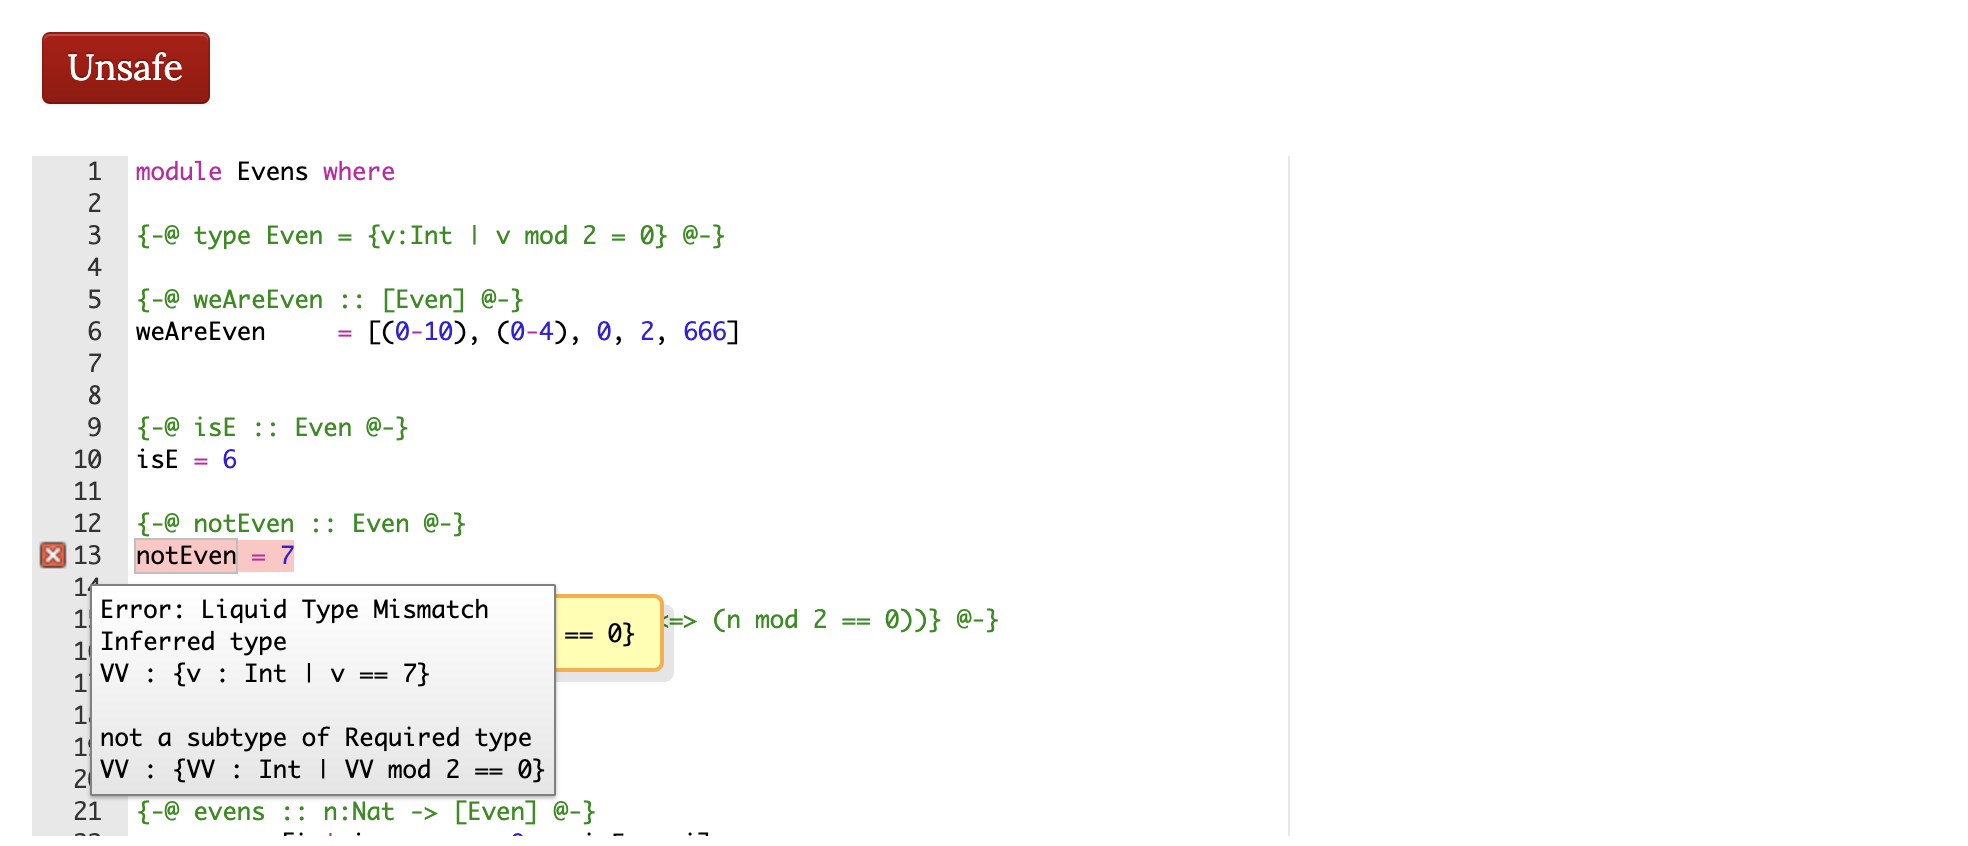
\includegraphics[scale=0.5]{assets/lh_demo_sm.PNG}
  \end{center}
  \caption{LiquidHaskell Demo using EvenInt}
  \label{fig:lh_demo}
\end{figure}

\par
Static refinement type checking is made possible in Haskell because of the lack 
of assignment statements. Once a variable $x$ is declared in a scope, its value 
cannot be changed. This allows SMT solvers to know precisely the value of $x$ 
and prove the refinement predicate statically. While I/O is possible in 
Haskell, their properties cannot be verified using LiquidHaskell.

\subsection{Idris}
\textit{Idris} \cite{idris} is a dependently typed functional language which first 
appeared in 2007. Idris bears similarity with Agda, both in terms of paradigm 
and type system. However they differ in one crucial way, Idris is designed to 
emphasise general purpose programming rather than theorem proving. In section 
\ref{section:agda}we stated that one of the less desirable property of 
Agda was its niche because of its emphasis in theorem proving. Idris provides 
interoperability with systems libraries and C programs, 
as well as language constructs for domain specific language 
implementation \cite{gpIdris}. 

\par
Syntactically Idris is very similar to Agda, dependent types are defined as so: 
\begin{figure}[H]
  \begin{lstlisting}      
    data EvenNat :  Nat -> Type where
      EvenZero  :: EvenNat 0
      EvenPlusTwo :: EvenNat n -> EvenNat (n + 2)
      
    data Vect : Nat -> Type -> Type where
      Nil  : Vect 0 a
      (::) : (x : a) -> (xs : Vect n a) -> Vect (n + 1) a
  \end{lstlisting}
  \caption{Dependent Types in Idris}
\end{figure}

\par
While Idris offers interoperability with multiple mainstream programming 
languages such as C and JavaScript, Idris remain predominantly a research tool. 
Idris is not production ready \cite{gpIdris} as it is missing certain libraries 
and more importantly nobody is working on Idris full time. Furthermore Idris is 
still a functional language, hence suffering from the limitation stated earlier. 

\section{Imperative Languages}

In this section we discuss dependent typing with regards to imperative 
languages. Imperative languages use the \textit{imperative programming} 
\cite{imperativeOverview} paradigm, in contrast to the functional 
programming, this paradigm emphasises \textit{how} a program will operate 
by using a series of statements to change the program state.

\par
Imperative languages can be further broken down into different categories, 
mainly Procedural and Object-Oriented. Many of the world's most popular languages 
fall into this two categories, C, FORTRAN, COBOL are examples of procedural 
languages while Java, C#, Kotlin are Object-Oriented Languages. Some languages such 
as C++, Python are multi-paradigm and allows the programmer to write code both 
in a procedural manner or object-oriented manner. 

\subsection{Research Languages}
Currently there are no production imperative programming language with 
native support for dependent types or refinement types. 
However, previous research has looked at creating languages with these 
capabilities or extending existing languages. In this section we will survey 
previous works in the area. 

\subsubsection{Ynot} \label{section:ynot}
\textit{Ynot} is an axiomatic extension to the \textit{Coq Proof Assistant} 
\cite{coq} created by Aleksandar Nanevski, et al \cite{ynot}. It adds 
support for writing and reasoning about dependently-typed 
programs with side-effects, i.e. written in an imperative manner. 

\par
The formal aspects of Ynot is based on \textit{Hoare Type Theory} \cite{htt}, 
a previous work by the authors and the concept of Monads, specifically 
the monadic system of Haskell. This allows Ynot to write 
ML or Haskell-style programs and still be able to formally 
reason about their values and effects.

\par
Ynot is publicly available for download on the homepage of the 
project \cite{theYnotProject} however it suffers from the same issues as 
Agda, Coq is a niche language and conventionally used as a theorem prover. 
Furthermore, the paper written on Ynot is theoretically complex, 
requiring prerequisite knowledge of advanced concepts such as Hoare 
Logic, Hoare Type Theory and Monads, making the paper challenging  
to new readers seeking to understand the concept of dependent types 
or refinement types in imperative languages. 

\subsubsection{Xanadu}
\textit{Xanadu} \cite{xanadu} is a dependently typed imperative language 
created by a team at the University of Cincinnati. The language was implemented 
in OCaml and is based on a previous project by the 
authors named \textit{Dependent ML} (DML) where the authors used a 
\textit{restricted form of dependent types} which essentially takes the 
form of refinement types.

\par
One aspect we found appealing in the paper is the use of real-world examples to 
show the concept of dependent types. The authors used examples such as binary 
search trees, array bound checking, etc to introduce the concepts, allowing new 
readers to easily understand the basic behaviour of these 
type systems. However, the Xanadu language described in the paper still uses many 
complex theoretical concepts that most readers are unlikely to be familiar with. 

\par
There are no examples of the actual language available online except some code 
snippets shown by the author in the original paper. As such we are unable to 
provide any analysis on the language itself. Xanadu was stated to be available 
online in the original paper, however the original cited webpage  
appears to have been taken offline. It is safe to conclude that the 
language itself is also no longer in active development. However, the 
language is worth a mention here as it shows the feasibility of 
imperative languages having dependent typing. The research by the authors 
are impressive and it serves as inspiration for our project. 

\subsubsection{Refined TypeScript}
\textit{TypeScript} is a superset of JavaScript that brings static typing to the 
language. A team from the University of California, San Diego wrote a paper \cite{rts} 
in 2016 showcasing Refined TypeScript (RSC), a lightweight refinement type 
system for TypeScript. 

\par
The key observation of RSC behaves like LiquidHaskell, it serves as a program 
verifier that verifies the refinement predicate using an SMT solver. However, 
unlike Haskell, Typescript is an imperative language and mutable is possible. 
The authors handled the mutable code in two ways, i) refinements are 
restricted to immutable variables and ii) reassignment is handled using 
Static single assignment (SSA) translation.

\par
The paper provides a unique way of handling assignment via SSA translation 
however this method introduces complexity into the design which are unnecessary 
in our project. We find this paper intriguing because of their idea of 
introducing refinement types in a mainstream programming language. 

\subsection{Refined Scala}
The \textit{Scala} \cite{scala} Programming Language is a statically 
typed multi-paradigm language, it is compiled into Java ByteCode and 
executed on the \textit{Java Virtual Machine}. 
As such, Scala shares similarity with Java and provides language 
interoperability. The Scala Type System is richer than the Java Type System, 
Scala supports certain types not available in Java such as Monads, 
Singleton Types, etc. Despite the rich type system, refinement types and dependent 
types are not native features of the language. However, an open source project 
named \textit{refined} \cite{refinedScala} has brought refinement types into Scala. 

\begin{figure}[H]
  \begin{center}
    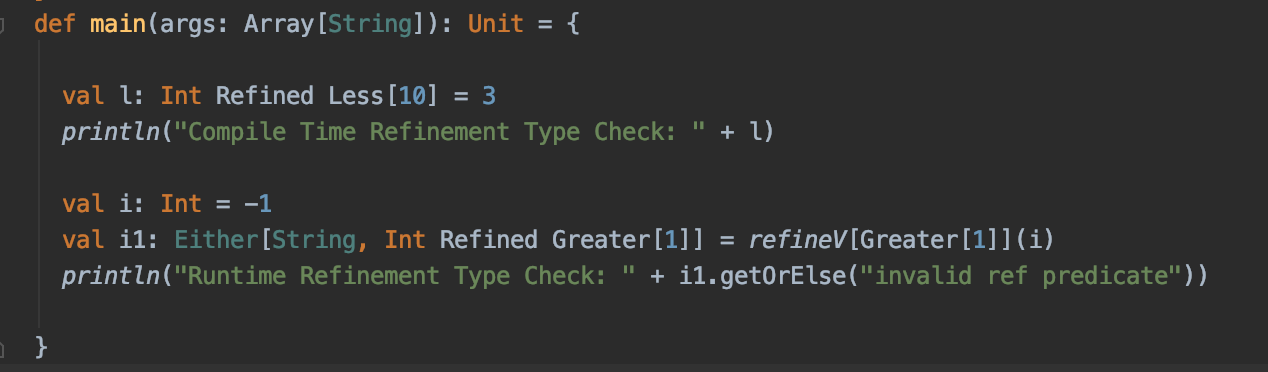
\includegraphics[scale=0.7]{assets/refined_scala.PNG}
  \end{center}
  \caption{Refinement Types in Scala using refined}
  \label{code:refined-scala}
\end{figure}

Figure \ref{code:refined-scala} is an example of refinement types using  
refined. While the library does not have a formal write up of its 
implementation and design decisions, the informal documentation is sufficient 
for us to identify and discuss multiple interesting design. 

\par
The first interesting observation we made is that the library does not allow 
refinement types with any arbitrary refinement predicate. Instead,  
the library has a set of predefined predicates one is able to associate 
with refinement types. In the example provided in figure \ref{code:refined-scala} 
we use the predicate \verb|Less[N]| to refine the integer type such that its value 
is always less than \verb|N|. As Scala is an imperative language where mutation 
is possible, the library insist that \verb|N| must be a 
literal and not a form of variable.

\par
Furthermore, in order to have compile time refinement type checking, one must 
initialise the variable of refinement type with a literal. Using the example 
in figure \ref{code:refined-scala}, the statement 
\verb|val l: Int Refined Less[10] = x| is forbidden as one tries to assign a 
refinement type a non-literal. 

\par
If one wishes to initialise a refinement type using a variable or function, one 
must use the \verb|refineV[P](v)| function, where \verb|P| is a predicate and 
\verb|v| is a value. The function will either give an error if \verb|v| does not 
satisfy \verb|P| or it gives the value \verb|v| which is refined using \verb|P|. 
An example of this use case in shown in figure \ref{code:refined-scala}.

\par
The refined Scala library provides a simple of using refinement types in a modern 
language through a restrictive manner. However, there are many design decisions 
one can take away from this project such as the combination of compile-time and 
runtime type checking. 

\subsection{C++ Templates} \label{section:cpp_templates}
\textit{C++ Templates} \cite{cppTemplate} are a way of passing the type of a 
data as a parameter so certain code can be reused. For instance, the same 
sorting algorithm can be used on multiple data types such as \textit{int} and 
\textit{double}, using templates the programmer will not need to write the same 
sorting function multiple times for different data types. 

\par
Templates are often compared to Java's \textit{Generics} \cite{javaGenerics} 
as the C++ equivalent. While this statement is mostly true, C++ templates 
differ in a big way. 
Generics only allow the template parameter to be a class, templates on the other 
hand allow the parameter to be a class, values or pointers. This feature allows 
one to create types that resembles refinement types. 

\par
C++ 11 introduced the notion of 
\textit{constexpr} and \textit{static\_assertion}. These allow for certain 
compile time checking, however the values checked must fulfill 
the \textit{constant expression} requirements \cite{cppConstExpr}. 

\begin{figure}[H]
  \begin{lstlisting}[language=c++]     
    template <int N, int M>
    struct LessThanN {
      const int value;
      LessThanN(): value(M) {
        static_assert(M < N, ``type is invalid'');
      }
    };
  \end{lstlisting}
  \caption{Compile Time Type Checking in C++}
  \label{code:compileLTN}
\end{figure}

\par
Figure \ref{code:compileLTN} shows a struct that represents a refined integer 
type whose values is can only be less than \verb|N|, defined as 
\verb|LessThanN<10, 5> x = LessThanN<10, 5>;|. Type checking is done at compile 
time using the \verb|static_assert| in the constructor. If one provides an 
invalid definition then a compile time error is thrown. 

\par
\verb|LessThanN<10, 12> x = LessThanN<10, 12>;| yields the following message: 
\par
\textbf{static\_assert failed due to requirement `12 $<$ 10' ``type is invalid''}

\par
Notice in our example we made the \verb|LessThanN| type immutable, the reason 
here is that there is no trivial way to ensure that if the programmer changes the 
value using \verb|x.value = 100| the new value coheres with the refinement 
type.

\subsubsection{Mutation of Template Variable}
In our previous example we have been passing an ``integer literal'' as the template 
parameter. Often programmers are required to 
work with varied values through variables, how will this effect the behaviour? 

\par
Consider the following hypothetical situation using the struct defined in 
figure \ref{code:compileLTN}: 

\begin{figure}[H]
  \begin{lstlisting}[language=c++]     
    int n = 5;
    LessThanN<n, 3> ltf = LessThanN<n, 3>();
    n = 2;
  \end{lstlisting}
  \caption{Mutating the Refinement Variable in C++}
\end{figure}

\par
Compiling the above code leads to a compile time error, C++ requires template 
arguments like $n$ above to be constant expressions. In order to use variables as template 
arguments, they have to be defined \textbf{const}. In which case the above 
situation is impossible as the variable $n$ now cannot be changed at line 3. 

\par
We see glimpses of refinement typing in C++, while it is still far from full 
refinement types. We are able to take note of certain mechanics such as ensuring 
variables associated with types are constant and the use of immutability. 

\section{Summary}
In this chapter we formally introduced dependent types and refinement types, 
these two type systems are similar in many aspect but are formally very 
different. Certain functional languages such as Agda and Idris have native support for 
dependent types however we observed that there is no imperative language with 
the same support. Research has attempted to bring dependent types and refinement types 
to imperative programming; these projects have been successful but the languages 
that are created is not widespread. 

\par
We found several open-source projects taht have attempted to bring refinement 
types to mainstream languages. We analysed \textit{refined}, a Scala based library that 
introduces refinement types to the language in a restrictive manner. We found the 
project interesting however it remains informal and lacks formal documentation. 
Finally, we studied C++ templates and notice the potential of introducing 
types that resembles refinement types.

\par
We identify that work in the area are missing in certain aspects, dependent types 
and refinement types are conventionally associated with functional languages 
because of the lack of mutation. Previous research that attempts to bring the more 
advanced type system to imperative languages remains mainly theoretical and 
does not relate to real-world languages. Practical projects that address 
these form of typing in real-world languages remains informal and are 
mainly documented as online articles. Our project will be focused on providing 
formal semantics for refinement types in a real-world imperative language. 

\chapter{Key Concepts in Programming Languages} \label{chapter:key_concepts}
Throughout our research, we observe certain ideas that commonly appear across 
different language constructs. In this chapter, we introduce three concepts, 
immutability, closures and hybrid type checking. We discuss these concepts 
in depth and identify how they relate to refinement types. These key ideas will 
be critical in the development of our language.

\section{Immutable Objects in Programming}
In this section we analyse the crucial differences between an immutable object   
and a constant in different programming lanaguages. We follow up our analysis by 
stating the importance of immutability and constancy with regards to type 
systems.

\subsection{Immutable vs Constant} \label{section:const_immutable}
\emph{Immutability} is an important concept in many programming languages, an 
object is immutable if its state cannot be modified after creation. 
\emph{Constancy} is often mistaken as an alternate name for 
immutability however they are two different concepts in programming languages. 
A constant is a variable that cannot be reassigned after initialisation, one can say 
that a constant is an immutable variable. 
The difference between an immutable object and a constant is subtle but crucial, 
these two notions does not provide the same guarantees that a value remains the 
same.
 
\par
Consider the following Java code in figure \ref{code:java_const}, 
assume a class \verb|Number| with a single field \verb|value| 
that is not \verb|final|.
\begin{figure}[H]
  \begin{center}
    \begin{tabular}{l}
      \verb|final Number n = new Number(10);| &
      \verb|n.value = 12;|
    \end{tabular}
  \end{center}
  \caption{Modifying Constant Reference in Java}
  \label{code:java_const}
\end{figure}

\par
In our simple example, we defined a constant \verb|n|, however the object held by 
\verb|n| is not immutable which allowed us to modify the 
value despite the variable \verb|n| being a constant. 

\par
C++ provides a more expressive form of constant where the previous example is not 
possible, however C++ allow a different scenario where the value of a constant 
can be changed. Consider the code snippet in figure \ref{code:cpp_const} 
where one declares a pointer \verb|p| that points to a constant integer. 
C++ ensures that one is not able to modify the value of \verb|&x| using 
the pointer \verb|p| however it does not guarantee \verb|x| cannot be 
modified in a different manner. The value pointed to by 
\verb|p| can change even though it is defined as a constant. 
\begin{figure}[H]
  \begin{center}
    \begin{tabular}{l}
      \verb|int x = 10;| &
      \verb|const int *p = &x;|&
      \verb|x = 5;|&
    \end{tabular}
  \end{center}
  \caption{Modifying Pointer to Constant in C++}
  \label{code:cpp_const}
\end{figure}

\subsection{Importance of Immutability}
The concept of immutability is fundamental and taught to new programmers early 
in the curriculum. However, the declration of constants are often introduced as 
a good software engineering practice that reduces careless errors in code. 
While it is a key use case of constants, they are often used to achieve a lot 
more. 

\par
Recall from section \ref{section:cpp_templates}, constants are used to enforce 
the behaviours of certain language features such as templates in C++. 
We see the same being done in Java's Lambda expression whereby any local variables 
referenced in the expression must be a constant. 

\par
Immutability is a key idea in our project as it is one of the biggest hurdle in 
bringing dependent types and refinement types into imperative programming. A 
good understanding the difference between constant and immutable proves to be a 
critical in the development of our language. Furthermore, we see how different 
imperative languages enforce constancy and immutability in areas where changes 
to variables are problematic. We identify the same idea can be incoporated into 
our language, enforcing immutable variables in refinement types. 

\section{Closures} \label{section:closures}
In this section we introduce the concept of closures using practical examples. 

\subsection{Introducing Closures}
In programming languages, \textit{Closures} are a way of enclosing functions 
with its surrounding environment, it allows a function to have access to local 
variables in the outer scope even if these variables have gone out of scope. 
Closures are present in many languages with first-class functions such as 
JavaScript, Python and Ruby. 

\begin{figure}[h]
  \begin{center}
    \begin{lstlisting}[language=C]
      function outer_function(x) {
          function inner_function(y) {
            return x + y;
          }
          return inner_function;
      }
      let closure = outer_function(10);
      closure(5); // 15
    \end{lstlisting}    
  \end{center}
  \caption{Closures in JavaScript}
  \label{code:clousure_js}
\end{figure}

Figure \ref{code:clousure_js} is an example of a function closure written in 
JavaScript. The function \verb|inner_function| is a closure as the variable 
\verb|x| from the outer scope is accessible within. The line 
\verb|let closure = outer_function(10)| binds the value 10 to \verb|x|, even after the 
\verb|outer_function| exits and \verb|x| is out of scope, the closure retains 
the value of \verb|x|.

\subsection{Closures in Types}
Closures are predominantly associated with functions, however the idea 
itself is useful more generally. The ability to bind values to variables 
within a scope can also be applied to types in order to preserve state and achieve 
a more consistent behaviour when performing type checking. 

\par
Recall that one of the difficulty of implementing refinement types in an 
imperative language is the presence of mutation. We propose that using the idea  
of closure one can prevent mutation to variables in a refinement type. For 
example, given the refinement type 
$\{\upsilon : int \text{ }|\text{ }\upsilon > x\}$, one can close $x$ within the 
type and independent of any changes to a different variable $x$ in the program. 
This idea is explored in depth further in the project.

\section{Hybrid Type Checking} \label{section:hybrid_type_checking}
Type checking can be difficult in programming languages with advanced features. 
In this section we introduce \emph{Hybrid Type Checking} \cite{hybridTypeChecking} 
as a combination of static and dynamic type checking. We show practical example 
of hybrid type checking in mainstream languages. Finally we propose a way of 
type checking refinement types using a hybrid type checking appraoch.

\subsection{Static and Dynamic Type Checking}
Programming languages handle type checking in two main ways, \textit{statically} 
and \textit{dynamically}. Static type checking is verifies the type 
safety of a program by analysing the program's text. Dynamic type checking 
verifies the same at runtime, after consideration the execution of statements. 

\par
One often associates strong and weak typing with static and dynamic type 
checking. While it is true that most weakly typed languages employ dynamic  
type checking, strongly typed languages do not exclusively use static typing. 
Modern programming languages offer complex features and some of which are hard 
or impossible to decide statically. In order to accomodate the evolving 
complexity of programming languages, the two distinct approachs are 
incorporated together. Gordon Plotkin, et al discussed the 
idea of dynamically checking a static language in this paper 
\cite{dynamicCheckStaticLanguage}. In practice, modern languages like 
Java and C# now supports the combination of static and dynamic type checking, 
e.g. Java's runtime checks for downcasting which will be 
discussed in the next subsection.

\subsubsection{Example of Hybrid Type Checking in Java} 
Downcasting is the act of converting a reference type of a base class to one of its 
derived class. However, unlike upcasting, downcasting is only possible if the 
variable of the base class is a value of the derived class being downcasted to. 
Discovering if a variable can be downcasted relies on dynamic runtime 
environment and thus it cannot be checked statically however there are certain 
properties about downcasting that can be checked statically. As such, 
Java employs a combination of static and dynamic checking 
to verify the type safety of this advanced feature. 

\par
Consider a program with three classes \verb|A|, \verb|B extends A| and 
\verb|C extends B|. The statements \verb|A x = new B();(C) x| 
type checks at compile time as there is a possibility it will succeed at 
runtime, however in this case it fails at runtime as \verb|x| is not a reference of 
type \verb|C|. Note that in other cases such as \verb|Integer i = 10; (String) i|, 
type checking fails at compile time because there is no way for the casting to 
succeed at all. The Java type checker verifies as much as possible 
statically, requiring only the most complicated type checks to be done at runtime. 

\subsection{Hybrid Type Checking in Refinement Types} \label{section:htc_ref}
Functional languages such as LiquidHaskell have shown the ability of type 
checking certain refinement types statically at compile time, however with the 
presence of mutation in imperative languages it turns out to be more difficult. 
The refinement predicate may contains variables whose value is only available 
at runtime or could have changed since declaration. This is an area that hybrid 
type checking proves to be useful. 

\par
Interestingly, Cormac Flanagan 
proposed a similar idea with the same name to verify the correctness of 
Dependent Types and Refinement Types 
in a $\lambda$-calculus \cite{hybridTypeChecking}. The paper 
inspired our idea by proposing a type checker that is 
``a synthesis of these two approaches that enforces precise interface 
specifications, via static analysis where possible, but also via 
dynamic checks where necessary''.

\par
Statically, we would not be able to verify that a value satisfy a refinement 
predicate, however we are able to verify some important properties. Consider the 
following example, $4 : \{\upsilon : int\text{ }|\text{ }\upsilon < x\}$, we 
cannot check the validity statically as the value of $x$ is not available. 
However, we can verify that there is a possibility for success. Similarly, we 
can verify some properties that will not succeed at all such as 
$\textit{false} : \{\upsilon : int\text{ }|\text{ }\upsilon < x\}$. This 
property can be easily checked by type checking the value against the base type. 
Interestingly, in certain cases refinement types can be completely checked 
statically. For example, $x : \{\upsilon : int\text{ }|\text{ }\upsilon < x\}$ 
does not type check, however in order to verify this statically one 
requires the help of automated theorem provers. In our project we have not 
consider these cases and left them as future work. 

\par
We propose that we can a use hybrid type checking technique to type check 
refinement types in an imperative language. We first statically verify that 
a value type checks against the base type, at runtime we verify that the 
refinement predicate holds. This idea is incorporated into our language 
and discussed in details further in the next chapter. 

\section{Summary}
In this chapter we introduced several key ideas in programming languages, 
explained the meaning behind them and how they relates to refinement types. 
We identified the difference between a constant and 
immutabile object which is key in the study of refinement types in 
imperative languages. We introduced the concept of closures and showed examples 
of it in action using JavaScript, we propsed a way of using closures 
in types that enables refinement types in imperative programming. 
We explained the difference in static 
and dynamic type checking, we followed up by observing how these two type 
checking mechanisms are combined in feature-rich langauges like Java in order to 
verify the correctness of complicated operations such as downcasting. Finally, 
we note that refinement types are difficult to verify statically and proposed 
using hybrid type checking to verify its safety. 

\chapter{The Simple-$R$ Language} \label{chapter:simple_r}
In this chapter we describe Simple-$R$, a basic procedural language 
with support for refinement types. We 
introduce certain ambiguous behaviour relating to refinment types and mutation. 
We extend the Simple-$R$ language with new variants that address these 
ambiguities using two approaches. Finally, we introduce dynamically  
allocated memory and discuss how this feature interacts with refinement types. 

\section{Language Syntax}
\begin{figure}[h]
  \begin{center}
    \begin{tabular}{l l l}
      \textit{Types} & $T$ & $:\text{ }int\text{ }|\text{ }bool\text{ }|
      \text{ }\{x: T\text{ }|\text{ }e\}$\\
      \textit{Function Type} &  & $:\text{ }T_1, T_2,T_3...T_n\longrightarrow T_0$\\
      \textit{Function Definition} & $f$ & $:$ $(x_0,x_1,...x_n) \longrightarrow C;e$ $|$ \\ 
      & & \; $(x_0,x_1,...x_n) \longrightarrow \textbf{begin } D;C;e\textbf{ end}$\\
      \textit{Operators} & $ops$ & $:$ $+$ $|$ $-$ $|$ $\wedge$ $|$ $\vee$ $|$ $<$ $|$ $>$ \\
      \textit{Expressions} & $e$ & $:$ $vals$ $|$ $x$ $|$ $e_1$ $ops$ $e_2$ 
      $|$ $f(e_1...e_n)$ \\
      \textit{Commands} & $C$ & $:$ $C_1;C_2$ $|$ \textbf{skip} $|$ $x\text{ }:= e_1$ 
      $|$ \textbf{while} $e_1$ \textbf{do} $C_1$ $|$ \\ 
        & & \; \textbf{if} $e_1$ \textbf{then} $C_1$ \textbf{else} $C_2$ $|$ 
        $\textbf{begin } D;C_1\textbf{ end}$ \\
      \textit{Declarations} & $D$ & $:$ $\textbf{var } x : T = e$ $|$ $D_0;D_1$\\
      \textit{Variables} & $vars$& $:$ $x \in {a,b,c...z}$\\
      \textit{Values} & $vals$& $:$ $\forall v \in \mathbb{Z}$ $|$ $\forall v \in \mathbb{B}$\\
      \textit{Variable Types Context} & $\Gamma$& $:$ $vars \mapsto T$\\
      \textit{Variable Values Context} & $\sigma$& $:$ $vars \mapsto vals$
    \end{tabular}
  \end{center}
  \caption{Language Syntax for Simple-$R$}
  \label{fig:simple_r_syntax}
\end{figure}

\par
Figure \ref{fig:simple_r_syntax} is the syntax of Simple-$R$, the paragraphs below 
explains the language in details. In contrast to other literature in this area, 
Simple-$R$ is a \textit{First Order Programming Language} \cite{FOL} modeled 
after the WHILE \cite{whileLanguage} programming language but with functions.
Rather than building it on the $\lambda$-calculus as one would in 
a Higher Order Language, we opted for a ``C-like'' syntax, with concepts such as 
expressions, commands and top-level functions. 
In order to achieve simplicity and observe the core behaviour of refinement 
types, the language is kept at a minimum with only the necessary construct. 

\paragraph{Types} The Simple-$R$ language has support the following four data types. 
\begin{itemize}
  \item The basic integer type \textit{int}
  \item The basic boolean type \textit{bool}
  \item The refinement type, written as $\{x: A\text{ }|\text{ }e\}$. This defines 
  a type that is a refinement of type $A$ that satisfies a boolean expression $e$.
\end{itemize}

\paragraph{Functions}
Functions Type are defined as $(T_1, T_2,T_3...T_n \longrightarrow T_0)$, 
it takes a up to $n$ types and returning a type. Note that functions are 
not first-class in this language, unlike a higher order 
language, functions types are its own entity and are distinct from the regular 
types. This distinction ensures that functions cannot be passed to 
other functions, nor can it return a function as a result. One can compare 
functions in Simple-$R$ to functions in C or Java. The function body is a 
command however it must end in an expression as the return value. Note that the 
return keyword is omitted. Functions return can be difficult to represent, in many 
languages functions can be terminated in certain branches using the 
return keyword. In order to achieve a simply model for functions, we came to 
the decision to disallow return in the middle of the function, values can 
only be returned at the very end of the function.

\paragraph{Operators}
The language supports the following built in operators.
\begin{itemize}
  \item Integer addition using the $+$ operator written in an infix notation.
  \item Integer subtraction using the $-$ operator written in an infix notation.
  \item Integer inequality $<$ as the less than operator.
  \item Integer inequality $>$ as the greater than operator.
  \item Logical conjunction using the $\wedge$ operator written in an infix 
  notation.
  \item Logical disjunction using the $\vee$ operator written in an infix 
  notation.
\end{itemize}

\paragraph{Expressions} The following expressions make up the language.
\begin{itemize}
  \item Variables and values represents the most basic form of an expression.
  \item The six operators which operates on two other expressions $e_1$ 
  and $e_2$ and return an expression.
  \item The function call $f(e_1..e_n)$ invokes function $f$ with arguments 
  $e_1..e_n$ and return the result. Functions are classified as expression as 
  one can utilise the computed result in other expressions. 
\end{itemize}

\paragraph{Commands} Commands are statements that can be executed to perform an 
actions. Simple-$R$ supports the following commands,
\begin{itemize}
  \item The assignment statement $(:=)$ assigns an expression $e_1$ to variable 
  $x$, note $x$ must have already been declared. 
  \item The \textbf{if then} and \textbf{while do} statements are the standard 
  control flow operations one would expect.
  \item The \textbf{skip} statement is use to indicate an empty expression and 
  does not perform any meaningful action. 
  \item The \textbf{begin ... end} command allows one to open a new scope. A 
  begin statement is followed by a variable declaration $D$, the declared 
  variable would then me accessible in the scope of command $C_1$. Upon reaching 
  \textbf{end}, the variable is out of scope and deallocated. 
\end{itemize}

\paragraph{Declarations} Declarations are the method one use declare new construct 
in the program. We start the language off having the most basic variable declaration 
$\textbf{var }x : T = e$ which declare a new variable $x$ of type $T$ and 
initialise it the resulting value of expression $e$. Multiple declarations can 
be declared in a scope by concatenating multiple declaration as $D_0;D_1$.

\paragraph{Variables and Values} In Simple-$R$, all variables are allocated 
locally, we use $x$ to denote a variable. Variables can take values as suggested by the types, all the integer 
literals $\mathbb{Z}$, booleans $\mathbb{B}$.

\paragraph{Variable Values Context} Variables are mapped to values in the program 
context $\sigma$. Each variable is allowed to only appear once in 
the context. We use \textbf{dom}($\sigma$) to retrieve the domain which represent 
the set of declared variables. We use the notation $\sigma(x)$ 
to retrieve the value bound to variable $x$.

\paragraph{Variable Types Context} Variables are also mapped to their types 
in the type context $\Gamma$. Each variable is allowed to only appear once in 
the context. This context will be used to type check the program using the 
typing judgement in the next section.

\section{Typing Rules}
This section defines the typing rules for the Simple-$R$ language. 
Throughout the text we will be extending the syntax defined in the 
previous chapter in order to accommodate more features. 
We will use the following metavariables and notations throughout our 
definitions.

\renewcommand\labelitemii{$\blacksquare$}
\begin{itemize}
  \item The metavariable $op$ as one of a range of operators. 
  \item The metavariable $v$ to range over all values.
  \item The uppercase letter $T$ to range over all types.
  \item Greek letters ($\alpha$, $\pi$, $\upsilon$) to define local variables in 
  the formula. 
  \item The following notations to operate on states. 
    \begin{itemize}
      \item $\sigma + \{x \mapsto v\}$ adds $\{x \mapsto v\}$ to $\sigma$ provided initially $x \notin\textbf{dom}(\sigma)$. 
      \item $\sigma[x \mapsto v]$ or $\sigma \uplus \{x \mapsto v\}$ updates $\sigma$ such that now $\sigma(x) = v$.
      \item $\sigma \setminus \{x\}$ to remove $x$ from $\sigma$, provided that $x \in \textbf{dom}(\sigma)$.
    \end{itemize}
  \item $\langle e, \sigma \rangle \Longrightarrow \langle e', \sigma \rangle$ as the transition relation for expression.
  \item $\langle C, \sigma \rangle \longrightarrow \langle C', \sigma' \rangle$ and $\langle C, \sigma \rangle \longrightarrow \sigma'$ as the transition relation for commands.
\end{itemize}

\par
We begin by defining the typing judgements. The typing judgements used in 
Simple-$R$ takes the form of the standard notation. 
\begin{center}
  $\Gamma \vdash e : T$\\
  $\Gamma \vdash_{C} C : void$\\
  $\Gamma \vdash_{D} D \dashv \Gamma'$\\
\end{center}
This first judgement represents that expression $e$ 
under the context $\Gamma$ has the type $T$. For a more consistent syntax, 
we use a pseudotype $void$ to represent that a command, the second judgement 
states that under environment $\Gamma$ the command $C$ is well-formed. 
The third states that a declaration produces the output context $\Gamma'$.

\par
Using the judgement rule we can easily define the fist few typing rules for base 
values \textit{int}, \textit{bool}, $nil$ and variables.

\begin{figure}[H]
  \begin{center}
    \begin{tabular} {c}
      $\forall n \in \mathbb{Z}$, $\Gamma \vdash n : int$ & 
      $\forall b \in \mathbb{B}$, $\Gamma \vdash b : bool$ & 
      $\Gamma \vdash_{C} \textbf{skip} : void$ & 
      $x : T, \Gamma \vdash x : T$ 
    \end{tabular}
  \end{center}
  \caption{Typing Rules for Base Values}
\end{figure}

\par
The remaining typing rules for the operators, statements and function  
calls are presented below. First we define the 
basic rules in figure \ref{fig:basic_typecheck}, 
most of the typing rule are straightforward and what one would expect from the 
type checker. 

\begin{figure}[H]
  \begin{center}
    \begin{tabular} {c}
      \inference {\Gamma \vdash e_1: int & \Gamma \vdash e_2: int}
        {\Gamma \vdash e_1 + e_2 : int}[(Op-Add)] \text{ }
      \inference {\Gamma \vdash e_1: int & \Gamma \vdash e_2: int} 
        {\Gamma \vdash e_1 - e_2 : int}[(Op-Minus)] & \\
      \inference {\Gamma \vdash e_1: int & \Gamma \vdash e_2: int}
        {\Gamma \vdash e_1 < e_2 : bool}[(Op-Less)] \text{ }
      \inference {\Gamma \vdash e_1: int & \Gamma \vdash e_2: int} 
        {\Gamma \vdash e_1 > e_2 : bool}[(Op-Greater)] & \\
      \inference {\Gamma \vdash e_1: bool & \Gamma \vdash e_2: bool}
        {\Gamma \vdash e_1 \wedge e_2 : bool}[(Op-And)] \text{ }
      \inference {\Gamma \vdash e_1: bool & \Gamma \vdash e_2: bool} 
        {\Gamma \vdash e_1 \vee e_2 : bool}[(Op-Or)] & \\
      \inference {\Gamma \vdash x: T & \Gamma \vdash e_1: T} 
        {\Gamma \vdash_{C} x := e_1 : void} [(Assign)] \text{ }
      \inference {\Gamma \vdash e_1: bool \\ \Gamma \vdash C_1: void & \Gamma \vdash C_2: void}
        {\Gamma \vdash_{C} \text{\textbf{if }} e_1 \text{\textbf{ then }} 
        C_1 \text{\textbf{ else }} C_2: void}[(If-Else)] & \\
      \inference {\Gamma \vdash e_1: bool & \Gamma \vdash C_1: void}
        {\Gamma \vdash_{C} \text{\textbf{while }} e_1 \text{\textbf{ do }} C_1 : void} [(While-Do)] \text{ }
      \inference {\Gamma \vdash C_0: void & \Gamma \vdash C_1 : void} 
        {\Gamma \vdash_{C} C_0;C_1 : T_2} [($C$-Concat)] 
        & \\
      \inference {\Gamma \vdash e_1: T_1} 
        {\Gamma \vdash_{D} \textbf{var } x : T_1 = e_1 \dashv \Gamma + \{x \mapsto T_1\}} [(D-$Vars$)] 
      & \\
      \inference {\Gamma \vdash_{D} D_0 \dashv \Gamma' & \Gamma' \vdash_{D} D_1 \dashv \Gamma''} 
        {\Gamma \vdash_{D} D_0;D_1 \dashv \Gamma''} [($D$-Concat)] \text{ }  
      & \\
      \inference {\Gamma \vdash D_1 \dashv \Gamma' & \Gamma' \vdash_{C} C_1 : void} 
        {\Gamma \vdash_{C} \textbf{begin }D_1;C_1\textbf{ end} : void} [(Begin)]     
    \end{tabular}
  \end{center}
\caption{Basic Typing Rules for Simple-$R$}
\label{fig:basic_typecheck}
\end{figure}

\subsubsection{Functions}
In order to type check a function we require access to the function signature, we define 
a mapping \textit{fts} $: f \mapsto T_1,T_2...T_n \longrightarrow T_0$ 
that allows us to retrieve the signature of a function. We first type check the 
function definition using the following new judgements.
\begin{center}
    $\Gamma \vdash_{f} (x_0,x_1...x_n) \longrightarrow C;e$\\
    $\Gamma \vdash_{f} (x_0,x_1...x_n) \longrightarrow \textbf{begin }D;C;e\textbf{ end}$
\end{center}

\par
Using the judgements, we check that the function definition matches the function 
signature using the rules in figure \ref{fig:type_check_f_def}.
\begin{figure}[H]
  \begin{center}
    \begin{tabular} {c}
      \inference{fts(f) = T_1,T_2...T_n \longrightarrow T_0 \\ 
      \Gamma \vdash x_0 : T_1 & \Gamma \vdash x_1 : T_1 & ... & \Gamma \vdash x_n : T_n \\
      \Gamma \vdash_{C} C : void & \Gamma \vdash e : T_0}{\Gamma \vdash_{f} (x_0,x_1...x_n) \longrightarrow C;e} [(Func-Def-$C;e$)]
      & \\
      \inference{fts(f) = T_1,T_2...T_n \longrightarrow T_0 \\ 
      \Gamma \vdash x_0 : T_1 & \Gamma \vdash x_1 : T_1 & ... & \Gamma \vdash x_n : T_n \\
      \Gamma \vdash_{D} D \dashv \Gamma' & \Gamma' \vdash_{C} C : void & \Gamma' \vdash e : T_0}
      {\Gamma \vdash_{f} (x_0,x_1...x_n) \longrightarrow \textbf{begin }D;C;e\textbf{ end}} [(Func-Def-$D;C;e$)]
    \end{tabular}
  \end{center}
  \caption{Typing Rules for Function Definitions}
  \label{fig:type_check_f_def}
\end{figure}

\par
We use first order logic to check that a $n$-nary function that takes 
the parameters $x_1$ to $x_n$ has the same types that is specified in the 
signature. Furthermore, we check that the function body is well formed and 
the returned expression matches the return type in the signature. 

\par
For a function call, we use the typing rule in figure \ref{fig:type_check_f_call}. 
If $f(e_1...e_n)$ is a $n$-nary function of type $T_1$ to $T_n$, 
then the arguments $e_1$ to $e_n$ must be of same type. 
Evaluation of the function will then satisfy the return type $T_0$ in the signature. 

\begin{figure}[H]
  \begin{center}
    \begin{tabular} {c}
      \inference {fts(f) = T_1,T_2...T_n \longrightarrow T_0 \\ 
      \Gamma \vdash e_1 : T_1 & \Gamma \vdash e_2 : T_2 &...& \Gamma \vdash e_n : T_n}
        {\Gamma \vdash f(e_1...e_n): T_0}[(Func-Call)]
    \end{tabular}
  \end{center}
  \caption{Typing Rules for Function Call}
  \label{fig:type_check_f_call}
\end{figure}

\subsubsection{Refinement Types} \label{section:ref_type_check}
Finally we define typing rules for a refinement types. A refinement type 
is represented in our system as $\{\upsilon : T\text{ }|\text{ }e\}$ and is 
constructed by a base type $T$ and a refinement predicate $e$ which may contain 
the free variable $\upsilon$ and any free variables in the program. A refinement 
type represent all values $\upsilon$ of $T$ where the expression $e[u/\upsilon]$ holds. 

\par
Recall that in section \ref{section:htc_ref} that we stated that the refinement 
predicate in general is undecideable at compile time and one requires dynamic 
checks for refinement types. However, we proposed that there are certain 
properties that can be checked statically such as a value must at least 
type checks against the base type for a chance of success. 

\par
We adopted a type checking approach that validates as much as possible 
statically and defers complicated type 
checking until runtime. In this section we will focus on static refinement type 
checking, we will discuss runtime type checking later in section 
\ref{section:runtime_refine}.

\par
We first define the typing rule for refinement types using the idea of 
\textit{universes} \cite{martinLof} in type theory, using the 4th judgement form 
$\Gamma \vdash A : Type$ to represent that $A$ is a type. 

\par
We begin by defining the formation rule for a refinement type. 
\begin{figure}[H]
  \begin{center}
    \begin{tabular} {c}
      \inference {\Gamma \vdash \upsilon : T & \Gamma, \upsilon : T \vdash e : bool}
        {\Gamma \vdash \{\upsilon : T\text{ }|\text{ }e\}: Type}[(Refine-Type-Form)]
    \end{tabular}
  \end{center}
  \caption{Typing Rules for Refinement Types in Simple-$R$}
\end{figure}

\par
We then define an \emph{unsound} typing judgement to capture this 
behaviour statically, soundness will be regained further on using dynamic checks.
\begin{figure}[H]
  \begin{center}
    \begin{tabular} {c}
      \inference {\Gamma \vdash e_1 : T}
      {\Gamma \vdash e_1 : \{\upsilon : T\text{ }|\text{ }e\}} [(Refine-Base-US)]
    \end{tabular}
  \end{center}
  \label{tj:unsound-refine}
\end{figure}

Additionally, we defining the typing rule for a subtypes, we express $A$ is 
a subtype of $B$ as $A \preceq B$. 
\begin{figure}[H]
  \begin{center}
    \begin{tabular} {c}
      
      $\Gamma \vdash \{\upsilon : T\text{ }|\text{ }e\} \preceq T$ (Subtype-Base 1)
      & \\
      \inference {\Gamma \vdash \forall \upsilon_1 : T.\text{ }e_1 \Rightarrow e_2[\upsilon_1/\upsilon_2]}
      {\Gamma \vdash \{\upsilon_1 : T_1\text{ }|\text{ }e_1\} \preceq \{\upsilon_2 : T_1\text{ }|\text{ }e_2\}} [(Subtype-Base 2)]
      & \\ 
      \inference {\Gamma \vdash T_1 \preceq T_2 & \Gamma \vdash T_1 \preceq T_3} 
      {\Gamma \vdash T_1 \preceq T_2} [(Subtype-Trans)]
      & \\
      $\Gamma \vdash T_1 \preceq T_1$ (Subtype-Reflex)
    \end{tabular}
  \end{center}
\end{figure}

\par
The four subtype rules defined above allows us to perform perform basic 
polymorphism. (Subtype Base 1 & 2) defines the basic definition of subtype. The 
first states that a refinement type of $T$ is trivially a subtype of $T$ and the 
second states that a refinement type $A$ is a subtype of another 
refinement type $B$ if the set of values in $A$ is a subset of or equal 
the values in $B$. (Subtype Trans) defines the transitivity of subtype and 
(Subtype Reflex) defines the reflexivity. 

\par
One should be able to use a value of type $T_1$ in a context 
expecting type $T_2$ provided $T_1$ is a subtype of $T_2$. For example, an 
expression $e$ of type containing all even natural numbers $EvenNat$ when passed 
to a context expecting a type $Nat$ should be valid. 

\par
We enable this behaviour using the judgement below.
\begin{figure}[H]
  \begin{center}
    \begin{tabular} {c}
       \inference {\Gamma \vdash T_1 \preceq T_2 & \Gamma \vdash e : T_1} 
      {\Gamma \vdash e : T_2} [(Subtype)]
    \end{tabular}
  \end{center}
\end{figure}

\par
In this section we covered the typing rules for Simple-$R$, typing rules are a 
way of allowing us to statically check the correctness of our program with 
regards to typing rules. Refinement types are hard to verify statically because 
of the dynamic behaviour when evaluating the refinement predicate. In the next 
section we will analyse the dynamic behaviour of the language. 

\section{Operational Semantics}
In this section we will define the \textit{Operational Semantics} 
\cite{operationalSemantics} for the Simple-$R$ language 
using the \textit{Structural Operational Semantics} \cite{plotkinSOS} (SOS) rules. 
\par
Figure \ref{fig:sos_expr} defines the reduction rules for the expressions in 
Simple-$R$. The rules for functions call will be covered in section 
\ref{section:functions_sos}.

\begin{figure}[H]
  \begin{center}
    \begin{tabular} {c}
      \inference {v = v_1 + v_2}{\langle v_1 + v_2, \sigma \rangle \Longrightarrow  \langle v, \sigma \rangle}[(Op-Add)] \text{ }
      \inference {v = v_1 - v_2}{\langle v_1 - v_2, \sigma \rangle \Longrightarrow  \langle v, \sigma \rangle}[(Op-Minus)]
      & \\
      \inference {v = v_1 < v_2}{\langle v_1 < v_2, \sigma \rangle \Longrightarrow  \langle v, \sigma \rangle}[(Op-Less)] \text{ }
      \inference {v = v_1 > v_2}{\langle v_1 > v_2, \sigma \rangle \Longrightarrow  \langle v, \sigma \rangle}[(Op-Greater)]
      & \\
      \inference {v = v_1 \wedge v_2}{\langle v_1 \wedge v_2, \sigma \rangle \Longrightarrow \langle v, \sigma \rangle}[(Op-AND)] \text{ }
      \inference {v = v_1 \vee v_2}{\langle v_1 \vee v_2, \sigma \rangle \Longrightarrow \langle v, \sigma \rangle}[(Op-OR)]
      & \\
      \inference {\langle e_1, \sigma\rangle \Longrightarrow \langle e_1', \sigma \rangle}
        {\langle e_1\text{ }op\text{ }e_2, \sigma  
        \rangle \Longrightarrow \langle e_1'\text{ }op\text{ }e_2, \sigma \rangle}[(Op-$E$ 1)]
      \text{ }
      \inference {\langle e_2, \sigma\rangle \Longrightarrow \langle e_2', \sigma \rangle}
        {\langle v\text{ }op\text{ }e_2, \sigma  
        \rangle \Longrightarrow \langle v\text{ }op\text{ }e_2', \sigma \rangle}[(Op-$E$ 2)]
      & \\
      \inference {x \in \textbf{dom}(\sigma)}{\langle x, \sigma \rangle \Longrightarrow \langle \sigma(x), \sigma \rangle}[(Vars)] 
    \end{tabular}
  \end{center}
  \caption{Basic Evaluation Rules for Simple-$R$ Expression}
  \label{fig:sos_expr}
\end{figure}

\par
Figure \ref{fig:sos_commands} defines the operational semantics for the 
basic commands in the language. The semantics for $\textbf{begin }D;C \textbf{ end}$ 
is complicated compared to the other commands and thus will be covered with more 
details in section \ref{section:scope_sos}.

\begin{figure}[H]
  \begin{center}
    \begin{tabular} {c}
      $\langle \text{\textbf{skip}}, \sigma \rangle \longrightarrow \sigma$ (Skip)
      \text{ }
      \inference {\langle C_1, \sigma \rangle \longrightarrow\sigma'}
        {\langle C_1;C_2, \sigma \rangle \longrightarrow \langle C_2, \sigma' \rangle}[(Cmd-Concat)]
      & \\
      $\langle \text{\textbf{if }\textit{true}} \text{\textbf{ then }} C_1 \text{\textbf{ else }} 
        C_2, \sigma \rangle \longrightarrow \langle C_1, \sigma\rangle$ (If-True)
      & \\
      $\langle \text{\textbf{if }\textit{false}} \text{\textbf{ then }} C_1 \text{\textbf{ else }} 
        C_2, \sigma \rangle \longrightarrow \langle C_2, \sigma\rangle$ (If-False)
      & \\
      \inference {\langle e_1, \sigma \rangle\Longrightarrow\langle e_1', \sigma \rangle}
        {\langle \text{\textbf{if }} e_1 \text{\textbf{ then }} C_1 \text{\textbf{ else }} 
        C_2, \sigma \rangle \longrightarrow \langle \textbf{if } e_1' \text{\textbf{ then }} C_1 \text{\textbf{ else }} 
        C_2, \sigma \rangle}[(IF-$E$)] 
      & \\
      $\langle \text{\textbf{while }} e_1 \text{\textbf{ do }} C_1, \sigma \rangle \longrightarrow \langle 
        \text{\textbf{if }} e_1 \text{\textbf{ then }} C_1;
        (\text{\textbf{while }} e_1 \text{\textbf{ do }} C_1) \text{\textbf{ else }} \textbf{skip}, \sigma \rangle$ (While)      
      & \\
      \inference {x \in \textbf{dom}(\sigma)} 
      {\langle x := v, \sigma \rangle \longrightarrow \sigma[x \mapsto v]} [(Assign-$V$)] \text{ }
      \inference {\langle e, \sigma \rangle \Longrightarrow \langle e', \sigma \rangle} 
      {\langle x := e, \sigma \rangle \longrightarrow \langle x := e', \sigma \rangle} [(Assign-$E$)]
     \end{tabular}
  \end{center}
  \caption{Operational Semantics for Simple-$R$ Commands}
  \label{fig:sos_commands}
\end{figure}

\subsection{Scoping} \label{section:scope_sos}
Scoping has an important role in programming languages, variables can be defined 
in scopes and are unavailable once outside. While there are many different 
variables that does not follow this rule, such as static variables and global 
variables. The design of Simple-$R$ supports only local variables which 
heavily relies on scoping. 

\par
In order to help us formalise the notion of scopes we define a new notation, 
$\Longrightarrow^{*}$ and $\longrightarrow^{*}$ as a multi-step evaluation. 
The evaluation rule $\langle e, \sigma \rangle \Longrightarrow^{*} 
\langle v, \sigma' \rangle$ simply 
evaluate the expression $e$ one or more times until it evaluates to a value $v$. 
The same applies for a multistep evaluation for commands, 
$\langle C, \sigma \rangle \longrightarrow^{*} \sigma'$ execute the command $C$ 
until there is no evaluation rules to apply. 

\par
Using a multi step evaluation, We can easily define the scoping rules as shown 
in figure \ref{fig:scoping_rules}.
  
\begin{figure}[h]
  \begin{center}
    \begin{tabular}{c}
      \inference {\sigma' = \sigma + \{x \mapsto v_0\} & x \notin \textbf{dom}(\sigma) 
      & \langle C_1, \sigma' \rangle \longrightarrow^{*} \sigma''} 
      {\langle\textbf{begin var }x : T = v_0; C_1 \textbf{ end}, \sigma \rangle 
      \longrightarrow \sigma'' \setminus \{x\}} [(Begin-$V$)] 
      & \\
      \footnotesize
      \inference {\langle e_1, \sigma \rangle \Longrightarrow \langle e_1', \sigma \rangle} 
      {\langle \textbf{begin var }x : T = e_1;C_1\textbf{ end}, \sigma \rangle 
      \longrightarrow \langle\textbf{begin var }x : T = e_1';C_1\textbf{ end}, \sigma \rangle} 
      [(Begin-$E$)]
      \normalsize
      & \\
      \inference {\sigma' = \sigma + \{x \mapsto v_0\} & x \notin \textbf{dom}(\sigma) 
      & \langle \textbf{begin }D_1;C_1 \textbf{ end}, \sigma' \rangle \longrightarrow^{*} \sigma''} 
      {\langle\textbf{begin var }x : T = v_0;D_1;C_1 \textbf{ end}, \sigma \rangle 
      \longrightarrow \sigma'' \setminus \{x\}} [(Begin-$D$-Concat-$V$)] 
      & \\
      \footnotesize
      \inference {\langle e_1, \sigma \rangle \Longrightarrow \langle e_1', \sigma \rangle} 
      {\langle \textbf{begin var }x : T = e_1;D;C_1\textbf{ end}, \sigma \rangle 
      \longrightarrow \langle\textbf{begin var }x : T = e_1';D;C_1\textbf{ end}, \sigma \rangle} 
      [(Begin-$D$-Concat-$E$)]
      \normalsize
    \end{tabular}
  \end{center}
  \caption{Scoping Rules for Simple-$R$}
  \label{fig:scoping_rules}
\end{figure}

\par
The \textbf{begin in} statement opens a new scope $\sigma'$ which 
assigns $x$ the value $v$, this scope allows the command $C_1$ to be evaluated 
using a multi step evaluation. Notice that the resulting state 
uses the $\setminus$ operator which removes all the variables 
in the set $\{x\}$ from the domain of $\sigma$. 

\par
This is necessary as it is possible to modify the range of $\sigma$ through 
assignments but not the domain. Upon exiting a scope the alteration to the program 
should still be visible, the only difference is that the variable $x$ is no longer in 
the state, i.e. has ran out of scope.

\par
The multi-step evaluation provides us to easily express scoping rules, 
the alternative would be to model an explicit call stack, which complicates the 
formulas and syntax.

\par
Concatenated declarations are handled by evaluating the declarations in order 
starting from the first. The rules (Begin-D-Concat-V) and (Begin-D-Concat-E) 
formalise the behaviour. To minimise space, in future text when we 
introduce new form of \textit{Declarations}, we will only 
be formalising the rules where only a single declaration is present. The 
corresponding concetenation rules, which can be derived easily using  
similar semantics to the ones used in in figure \ref{fig:scoping_rules}, 
are omitted.

\subsection{Function Calls} \label{section:functions_sos}
Functions in imperative language often operates in their own scope, they 
do not have the access to the local variables out of their scope however 
one can pass data using arguments. Functions in Simple-$R$ are call by values, 
changing the value of an argument in the function does not change the value in 
the outside scope. Our multi-step evaluation rule defined previously helps us 
evaluate functions in their own scope. 

\par
In order to define the operational semantics of a function we will need to 
specify the function body. We define a mapping 
\textit{fns} $: f \mapsto ((x_1, x_2...x_n), f_{body})$ where $f_{body}$ can either 
be $C;e$ or $\textbf{begin }D;C;e\textbf{ end}$, 
using this mapping we can retrieve the body of a function. Since functions 
definition cannot be changed at runtime, this does not need to be part of the 
configuration and can be consider as a static context.

\par
We first define the rules for the simple case where the function body is simply 
$C;e$, the rules for $\textbf{begin }D;C;e\textbf{ end}$ will be defined later 
in the section. 
\begin{figure}[H]
  \begin{center}
    \begin{tabular} {c}
      \inference {\textit{fns}(f) = ((x_1..x_n), C;e) & \langle C, \sigma' 
      \rangle \longrightarrow^{*} \sigma''
        \\ \sigma' = \{x_1 \mapsto v_1 ... x_n \mapsto v_n\} & \langle e, \sigma'' \rangle \Longrightarrow^{*} \langle v, \sigma'' \rangle}
      {\langle f(v_1...v_n), \sigma \rangle \Longrightarrow \langle v, \sigma \rangle} [(Func-$V$)]
      & \\
      \inference {\langle e_k, \sigma \rangle \Longrightarrow \langle e_k', \sigma' \rangle}
      {\langle f(v_0...v_{k - 1},e_k...e_n), \sigma \rangle \Longrightarrow \langle f(v_0...v_{k - 1}, e_{k}'...e_n), \sigma \rangle} [(Func-$E$)]
    \end{tabular}
  \end{center}
  \caption{Basic Functions Semantics for Simple-$R$}
  \label{fig:basic_functions}
\end{figure}

\par
Figure \ref{fig:basic_functions} shows the basic evaluation rules for functions,  
the first rule (Func-$V$) creates a new state where only 
the argument values are available. We then evaluates the function body until it 
evaluates to a value which is then returned to the caller's context. Unlike 
scopes, functions only update its local state which is dellalocated upon return. 
It cannot change the caller's state. 

\par
The second rule (Func-$E$) evaluates the expression passed into the 
function as arguments. Our language defines a strict behaviour that all 
arguments are evaluated in the order they are passed in the order they are listed, 
i.e. from left to right and arguments are call-by-value as in languages like 
Java and ML but not like C or Haskell. 

\par
In certain cases one might declare new local variables in functions and 
subsequently use these local variables in the return expression. Figure 
\ref{fig:declaration_functions} defines the rules for this behaviour. 

\begin{figure}[h]
  \begin{center}
    \begin{tabular} {c}
      \inference {
      \langle C, \sigma \rangle \longrightarrow^{*} \sigma' & \langle e, \sigma' \rangle \Longrightarrow^{*} v}
      {\langle \textbf{begin }C;e\textbf{ end}, \sigma \rangle \Longrightarrow \langle v, \sigma' \rangle} [(Func-Body)]
      & \\
      \inference {\sigma' = \sigma + \{x \mapsto v_0\} & x \notin \textbf{dom}(\sigma) \\
      \langle \textbf{begin }C;e\textbf{ end}, \sigma' \rangle \Longrightarrow^{*} \langle v, \sigma'' \rangle}
      {\langle \textbf{begin }x : T = v_0;C;e\textbf{ end}, \sigma \rangle \Longrightarrow \langle v, \sigma'' \rangle} [(Func-Body-$D$)]
      & \\
      \inference {
      \sigma' = \sigma + \{x \mapsto v_0\} & x \notin \textbf{dom}(\sigma) \\
      \langle \textbf{begin }D;C;e\textbf{ end}, \sigma' \rangle \Longrightarrow^{*} \langle v, \sigma'' \rangle}
      {\langle \textbf{begin }x : T = v_0;D;C;e\textbf{ end}, \sigma \rangle \Longrightarrow \langle v, \sigma' \rangle} [(Func-Body-$D$-Concat)]
      & \\
      \inference {
      \textit{fns}(f) = ((x_1..x_n),\textbf{begin }D;C;e\textbf{ end}) 
      \\ \sigma' = \{x_1 \mapsto v_1 ... x_n \mapsto v_n\} & 
      \langle \textbf{begin }D;C;e\textbf{ end}, \sigma' \rangle \Longrightarrow^{*} v}
      {\langle f(v_1...v_n), \sigma \rangle \Longrightarrow \langle v, \sigma \rangle} [(Func-$D$)]
    \end{tabular}
  \end{center}
  \caption{Semantics for Declarations in Functions}
  \label{fig:declaration_functions}
\end{figure}

\par
The first three rules in the figure behave similar to the 
operational semantics for \textbf{begin end}, however, instead of simply 
returning the state, we return the value of the return expression. 
Note that in order to minimise space, we ommited the rule where an expression 
is used in the declaration, however one can easily derived the rule using 
(Begin-E) and (Begin-D-Concat-E) from figure \ref{fig:scoping_rules}. 
Finally, the rule (Func-$D$) ties everything together by specifying the rules 
for evaluating a function where the body contains new variable declarations. 

\subsection{Runtime Refinement Type Checking} \label{section:runtime_refine}
A declaration of a variable that is a refinement type requires specific 
evaluation rules. When one declares a variable of a refinement type, the language 
has to ensure that the refinement predicate evaluates to true. While we have 
defined a statically typed language, even in a statically typed language, 
there are cases when the type of some data cannot be determined statically as 
discussed in section \ref{section:hybrid_type_checking}.

\par
In section \ref{section:ref_type_check} we demonstrated how basic properties 
of refinement types are checked statically in Simple-$R$ using 
the unsound typing judgement (Refine-Base-US), now we show 
how these refinement types are validated dynamically in order to regain soundness. 
We define a special form of typing judgement to type check refinement types 
dynamically.

\begin{figure}[H]
  \begin{center}
    \begin{tabular} {c}
      $\sigma, \Gamma \vdash_{R} e_1 : \{\upsilon : T \text{ }|\text{ }e\}$
    \end{tabular}
  \end{center}
  \caption{Typing Judgement for Refinement Types}
  \label{fig:refine_judgement}
\end{figure}

\par
Figure \ref{fig:refine_judgement} shows a typing judgement for refinement 
types which has the ability to access the runtime state $\sigma$. We can then 
perform a type check on refinement type using the rule defined below. 

\begin{figure}[H]
  \begin{center}
    \begin{tabular} {c}
      \inference{\Gamma \vdash e_1 : T_1 & \langle e[e_1/\upsilon], \sigma \rangle \Longrightarrow^{*} \langle \textit{true}, \sigma \rangle}
      {\sigma, \Gamma \vdash_{R} e_1 : \{\upsilon : T_1\text{ }|\text{ }e\}} [(Runtime-Refine)]
    \end{tabular}
  \end{center}
  \caption{Type Checking Refinement Types}
  \label{fig:refine_typecheck}
\end{figure}

\par
During runtime, the typing judgement in figure \ref{fig:refine_typecheck} 
asserts that an expression $e_1$ is a valid refinement type if it 
evaluates to the base type $T_1$ and the refinement predicate $e[e_1/\upsilon]$ 
evaluates to true under state $\sigma$.

\par
Our type check rule looks to capture the behaviour of refinement type however it 
turns out the current definition is underspecified in the presence of mutation. 
In the next section we will put forward certain ambiguities with the 
design and discuss different choices one can make to address them.

\section{Refinement Types and Variables}
\subsection{Ambiguity of Refinement Types involving Mutation}
Programming languages often have a wide range of features, often the team behind 
the language have to put extensive thought into the design decisions. As there 
are often multiple way to handle a certain feature, rarely is there a definite 
answer to which is the most optimal, often they are a matter of human judgement 
or aesthetics. 

\par
This problem is known as \textit{feature interactions} 
\cite{featInteract}, it describes the problem in some situations multiple 
features would modify the behaviours of each others. The same applies to 
refinement types, which can be seen as a feature. For instance, the inclusion 
of refinement types would modify the behaviour of assignments and vice versa. 
This section will cover the different ways of handling refinement types and how 
they interact with other features.
Consider these few ambiguity of using variables to define dependent types. For 
instance: 

\begin{figure} [H]
  \begin{tabs}{1cm,2cm}
    \textbf{begin var }$y\text{ }:\text{ } int = 10;$ \\
    \tab\textbf{begin typedef }$BoundedIntY$ = $\{i : Int\text{ }|\text{ } i < y\}$; \\ 
    \tab\tab\textbf{begin var }$x\text{ }:\text{ }BoundedIntY = 4;y := 5$\textbf { end} \\
    \tab\textbf {end} \\
    \textbf{end}
  \end{tabs}  
  \caption{Mutation to Free Variables in Refinement Predicate}
  \label{fig:amb_refinement_vars}
\end{figure}

\par
The simple program demonstrated in figure \ref{fig:amb_refinement_vars} declares a 
bounded integer type $BoundedIntY$ whose value cannot be greater than another integer $y$, 
a free variable in the program. A variable $x$ is declared to be of type 
$BoundedIntY$ with the appropriate value. Later in the program, the value of $y$ 
changes. resulting to $x$ now being ill-typed. The behaviour is now undefined, 
should $x$ still be well-typed, or is the behaviour invalid? This section 
discusses the problem in detail. 

\subsection{Type Declaration}
First we need to introduce a new declaration statement for type declaration, 
in the example above we used the statement 
(\textbf{typedef} $x = \{\upsilon : T\text{ }|\text{ }e\}$) to denote a 
new refinement type $\{\upsilon : T\text{ }|\text{ }e\}$ with the name $x$. It is 
important to note that a \textbf{typedef} can only declare a new refinement type, one is 
not able to use \textbf{typedef} to provide an alias for a base type, the type 
definition $\textbf{typedef } x = int$ is forbidden, however one is able to achieve the 
same effect by declaring $\textbf{typedef }newint = \{\upsilon : int\text{ }|\text{ }true\}$.

\par
Figure \ref{fig:typedef-extend} extends the syntax of Simple-$R$ to introduce 
the new form of declaration.
\begin{figure}[H]
  \begin{center}
    \begin{tabular} {l l l}
      \textit{Declaration} & $D$ & $:$ ... $|$ \textbf{typedef }$x = \{\upsilon : T\text{ }|\text{ }e\}$\\
      \textit{Variable Types Context} & $\Gamma$& $:$ $vars \mapsto T\text{ }|\text{ }Type$\\
      \textit{Type Name Context} & $\tau$& $:$ $vars \mapsto \{\upsilon : T\text{ }|\text{ }e\}$ \\
    \end{tabular}
  \end{center}
  \caption{Type Name Context Extension for Simple-$R$}
  \label{fig:typedef-extend}
\end{figure}

\par
In our syntax, we have a context mapping $vars$ to $vals$, We now need to 
add a similar mapping for types, We use $\tau$ to represent the type name map. 
We modified our Variable Types Context so that we can identify if a certain 
variable is a value or a type. 

\par
The typing judgement has to be updated to accommodate type checking using a 
declared type. All typing judgements are updated from $\Gamma \vdash e : T$ to 
$\Gamma, \tau \vdash e : T$.

\begin{center}
  \begin{tabular} {c}
    \inference{\Gamma \vdash \{\upsilon : T\text{ }|\text{ }e\} : Type}
    {\Gamma, \tau \vdash_{D} \textbf{typedef } x = \{\upsilon : T\text{ }|\text{ }e\} 
    \dashv \Gamma + \{x \mapsto Type\}, \tau + \{x \mapsto \{\upsilon : T\text{ }|\text{ }e\}\}} [(Typedef)]
  \end{tabular}
\end{center}

\par
As a declared type is only ever a refinement type, we established that they cannot 
be type checked statically. However, we must still validate the 
static refinement type (Refine-Base-US) rule using the following judgement.

\begin{center}
  \begin{tabular} {c}
    \inference{\Gamma, \tau \vdash y : Type & \Gamma, \tau \vdash x : \tau(y)}
    {\Gamma, \tau \vdash x : y} [(Refine-Base-Vars-US)]
  \end{tabular}
\end{center}

\par
During runtime, the type is validated using the following rule.
\begin{figure}[H]
  \begin{center}
    \begin{tabular} {c}
      \inference{\Gamma \vdash x : Type & \Gamma \vdash_{R} e_1 : \tau(x)}
      {\sigma, \Gamma \vdash_{R} e_1 : x }[(Runtime-Refine-Vars)]
    \end{tabular}
  \end{center}
\end{figure}

\par
In our operational semantics, our configurations is updated from 
$\langle C, \sigma \rangle$ to $\langle C, \sigma, \tau \rangle$ in order to 
incorporate this new feature. 
All previous operational semantics should be updated consistently.

\begin{figure}[H]
  \begin{center}
    \begin{tabular} {c}
      \inference { 
      \langle C_1, \sigma, \tau' \rangle \longrightarrow \langle \sigma', \tau' \rangle\\
      x \notin \text{\textbf{dom}}(\sigma) & x \notin \textbf{dom}(\tau) & \tau' = \tau + \{x \mapsto \{\upsilon : T\text{ }|\text{ }e\}\}}
      {\langle \textbf{begin typedef }x = \{\upsilon : T\text{ }|\text{ }e\};C_1\textbf{ end}, 
      \sigma, \tau \rangle \longrightarrow 
        \langle \sigma', \tau \rangle} [(Type-$D$)]
    \end{tabular}
  \end{center}
\end{figure}

\par
Note that unlike the rule for variable declaration, we did not have to remove 
the type name $x$ from the context after evaluation. This is because unlike 
variables, types cannot change after declaration. The new type simply goes 
out of scope, hence the new type context will simply be our initial one. 

\par
The operational semantic above simply adds a new type definition with name $x$ 
into the Type Name context $\tau$. Importantly, the variable $x$ cannot have 
already been defined as a value variable in $\sigma$ and a type of the same name 
can not already be defined. Logically it is equivalent to the semantics for 
variable declaration.

\subsection{Complete Immutability}
The main issue one encounters when associating refinement types with imperative 
languages is the presence of mutability and assignments. The obvious way to 
work around this problem is to remove the ability to make changes to the state 
of the program, all variables declared are final.

\par
Using this approach does definitely resolves the uncertainty the usability of 
the language is poor. Imperative programming relies on state changes, forbidding 
that goes against the paradigm. However, if we strategically enforce immutability 
we can resolve the ambiguity while preserving a flexible imperative style 
language. In the next few sections we will discuss two approaches that 
improve the specification of our type checker through restricting changes to 
variables. 

\subsection{Immutability in Refinement Types}
In order to avoid feature interaction between refinement types and assignments, we 
observe that it is suffice to require free variables appearing in a refinement 
predicate to be immutable. This approach improves flexibility of our language as 
one will still be able to have mutability in context irrelevant to refinement 
types. In this section we extends Simple-$R$ with this functionality and dubbed 
the new variant Simple-$R_{I}$.

\par
In order to capture the notation of immutable types, the set of variables $vars$ 
is partitioned into two different distinct categories. Mutable and immutable, we 
define a predicate $is\_immutable$ that specify if a given variable is immutable. 
$is\_immutable(x)$ holds if and only if $x$ is immutable. 

\begin{figure}[H]
  \begin{center}
    \begin{tabular} {l l l}
      \textit{Declaration} & $D$ & $:$ $...\text{ }|\text{ }\textbf{const }x : T = e_1$
    \end{tabular}
  \end{center}
  \caption{Immutable Variable Context for Simple-$R_{I}$}
\end{figure}
 
One can declare an immutable variable similar to defining a mutable 
variable, using the \textbf{const} $x : T = e$ statement. We establish the following 
rules for immutable variables. 

\par
The typing judgement appears in analogous to that of variable declaration 
using $\textbf{var}$. 
\begin{center}
  \begin{tabular} {c}
    \inference {\Gamma \vdash e_1: T_1} 
        {\Gamma \vdash_{D} \textbf{const } x : T_1 = e_1 \dashv \Gamma + \{x \mapsto T_1\}} [(Const-$D$)]
  \end{tabular}
\end{center}

\par
The operational semantics in figure \ref{fig:immu_rules} describes the process of 
declaring an immutable variable, the semantics are similar to that of  
mutable variables. The only new addition here is extending the assignment 
statement to only accept the latter. 

\begin{figure}[h]
  \begin{center}
    \begin{tabular}{c}
      \inference {
      \langle C_1, \sigma', \tau \rangle \longrightarrow^{*} \langle \sigma'', \tau' \rangle 
      \\ \sigma' = \sigma + \{x \mapsto v\} & x \notin \textbf{dom}(\sigma)} 
      {\langle \textbf{begin const }x : T = v;C_1\textbf{ end}, \sigma, \tau \rangle 
      \longrightarrow \langle \sigma'' \setminus \{x\}, \tau' \rangle} [(Begin-$C$)] 
      & \\
      \footnotesize
      \inference {\langle e_1, \sigma, \tau \rangle \Longrightarrow \langle e_1', \sigma, \tau \rangle} 
      {\langle \textbf{begin const }x : T = e_1;C_1\textbf{ end}, \sigma,\tau \rangle 
      \longrightarrow \langle \textbf{begin const }x : T = e_1';C_1\textbf{ end}, \sigma, \tau \rangle}
      [(Begin-Const-E)]
      \normalsize
      & \\
      \inference {
      \langle \textbf{begin }D_1;C_1\textbf{ end}, \sigma', \tau \rangle \longrightarrow^{*} \langle \sigma'', \tau' \rangle 
      \\ \sigma' = \sigma + \{x \mapsto v\} & x \notin \textbf{dom}(\sigma)} 
      {\langle \textbf{begin const }x : T = v;D_1;C_1\textbf{ end}, \sigma, \tau \rangle 
      \longrightarrow \langle \sigma'' \setminus \{x\}, \tau' \rangle} [(Begin-Concat-$C$)] 
      & \\
      \inference {x \in \textbf{dom}(\sigma) & \neg is\_immutable(x)} 
      {\langle x := v, \sigma, \tau \rangle \longrightarrow \langle \sigma[x \mapsto v], 
      \tau \rangle} [(Assign-$C$)]
    \end{tabular}
  \end{center}
  \caption{Immutable Variables Rules for Simple-$R_{I}$}
  \label{fig:immu_rules}
\end{figure}

\par
Once we define the ability to define immutable variables, we can utilise it in 
our type definition. First we refine our specification for \textbf{typedef} 
with regards to refinement types using the evaluation rules.

\par
We require a new notation to capture all the variables that appear in an 
expression $e$, we use the notation \textit{free\_vars}$(e)$ to give the set of all 
variables that appear in an expression $e$.

\par
Notice that in our syntax the refinement predicate is simply a boolean 
expression, this means that it is not possible for the refinement predicate to 
declare any new variables within it. So it is easy to see that for a refinement 
predicate $e$, we require $\textit{free\_vars}(e) \subseteq \textbf{dom}(\sigma)$.

\par
Using the new notation we can easily verify that all free variables in a 
refinement predicate $is\_immutable$ using the evaluation defined below. The same 
applies when one declare a variable of type $\{\upsilon : T\text{ }|\text{ }e\}$ 
without using the \textbf{typedef} command.

\begin{figure}[h]
  \begin{center}
    \begin{tabular}{c}
      \inference {
      x \notin \text{\textbf{dom}}(\sigma) & x \notin \textbf{dom}(\tau) \\
      \forall \alpha \in \textit{free\_vars}(e).\text{ }is\_immutable(\alpha)
      \\ \langle C_1, \sigma, \tau + \{x \mapsto \{\upsilon :T\text{ }|\text{ }e\}\} 
      \rangle \longrightarrow \langle \sigma', \tau \rangle}
      {\langle \textbf{begin typedef } x = \{\upsilon :T\text{ }|\text{ }e\};C_1\textbf{ end}, 
      \sigma, \tau \rangle \longrightarrow 
        \langle \sigma', \tau \rangle} [(Refine-Typdef-Immu)]
      & \\
      \inference {
      x \notin \text{\textbf{dom}}(\sigma) & x \notin \textbf{dom}(\tau) \\
      \forall \alpha \in \textit{free\_vars}(e).\text{ }is\_immutable(\alpha)
      \\ \langle C_1, \sigma + \{x \mapsto v_1\} , \tau
      \rangle \longrightarrow \langle \sigma', \tau \rangle}
      {\langle\textbf{begin var }x : \{\upsilon : T\text{ }|\text{ }e\} = v_1;C_1 \textbf{ end}, \sigma, \tau \rangle 
      \longrightarrow \langle \sigma' \setminus \{x\}, \tau \rangle} [(Refine-Immu)]
    \end{tabular}
  \end{center}
\end{figure}

\par
We now address the ambiguity brought up using this semantic. The program in figure 
\ref{fig:amb_refinement_vars} is no longer a valid program as 
$y$ is a mutable variable and is forbidden from appearing in a refinement type. 
One would have to rewrite the declaration of $y$ using \textbf{const} which 
forbids it from being assigned to after initialisation. 
It is easy to see by restricting free variables in the refinement predicate we ensure 
that the expression stays the same throughout its existence, avoiding any 
complications regarding mutation.

\par
The approach laid out here is a simple approach to dealing with the ambiguity of 
having mutability and refinement types. Interestingly, C++ utilises the same 
strategy for templates values, where a value passed into a template must be a 
constant expression. 

\par
We could potentially adapt a clever approach used by the Java programming 
language to overcome variable mutation in Anonymous classes. Java requires that 
any variables accessed by an anonymous class that is part of 
its enclosing scope to be final or \textit{effectively final} 
\cite{effectFinal}. An effectively final variable is a variable that is not 
declared immutable but its value is not changed after declaration. While this 
does improves some flexibity as one do not need to use the \textbf{const} 
statement for declaration, it behave the same for all intents and purposes. 
For this reason we consider this additional feature as future consideration and 
out of scope for this current project. 

\par
The limitation of this approach is of course the fact that one has to strategically 
declare the variables needed, in some cases one might not be able to declare 
immutable variable but still want the ability to define a refinement type.

\subsection{Type Closure}
If we further analyse our design, we notice that our main concern is for the 
refinement predicate to stay static, any changes in the program context should 
not change its definition. In this section, we propose a design based on closures 
which allows us to ensure the values of variables in a refinement predicate remain 
constant without the need of declaring constant variables. We define a new variant of 
Simple-$R$ named Simple-$R_{C}$ that extends the former and implements this 
technique to handle refinement types. 

\par
Recall in section \ref{section:closures} we introduced the idea of closures, a 
closure is simply a function enclosed with an environment. Closures have access to 
variables from the calling context, even if the original variable goes out of 
scope. A value is bound to the variable in the closure such that changes does 
not reflect within. In order to make free variables in a predicate independent, 
we designed a similar approach where we \emph{snapshot} variables, i.e. 
bind free variables to a value. We name this approach of closing 
variables used in types as \emph{Type Closure}. 

\par
Taking the example program in figure \ref{fig:amb_refinement_vars} if the 
value of variable $y$ in the refinement predicate is snapshotted at the time of 
creation, then any changes to the variable $y$ will not 
affect the type definition and the program will stay well typed.

\par
Semantically, closures can be modeled as a data structure mapping 
functions to environment as demonstrated in the extended lambda calculus proposed by 
Gerald J. Sussman and Guy L. Steele Jr in this paper \cite{closureLambdaOp}. We 
adapted a similar approach, however instead of a function mapping to an 
environment, we have a type mapping to an environment. We modify the 
definition of $\tau$ to hold this information.

\begin{center}
   \begin{tabular} {c c c}
     \textit{Type Name Context} & $\tau$& $:$ 
     $vars \mapsto (\{\upsilon : T\text{ }|\text{ }e\}, \sigma, \tau)$ \\
   \end{tabular}
\end{center}

The Type Name Context now associate a refinement type with its 
evaluation context. The said context is simply the $\sigma, \tau$ at the time of 
the refinement type creation. 
We define $\sigma_1$ and $\tau_1$ as a copy of the program state $\sigma$ and 
$\tau$ and attach this to the type. 

\begin{figure}[H]
  \begin{center}
    \begin{tabular} {c}
      \inference {\sigma_1 = \sigma & \tau_1 = \tau
      \\ \langle C_1, \sigma, \tau + \{y \mapsto (\{\upsilon : T\text{ }|\text{ }e\}\}, \sigma_1, \tau_1)
      \rangle \longrightarrow^{*} \langle \sigma', \tau\rangle}
      {\langle\textbf{begin typedef } y = \{\upsilon : T\text{ }|\text{ }e\};C_1\textbf{ end}, 
      \sigma, \tau \rangle \longrightarrow \langle \sigma', \tau \rangle} [(Refine-Typedef-Closure)]
    \end{tabular}
  \end{center}
  \caption{Evaluation of Refinement Type with Closures}
\end{figure}

\par
In order to type check refinement types with closures, we update our typing 
judgement for refinement type. Notice that we would only require type 
closures for named types; if one declares a refinement type without a name i.e.  
$\textbf{var }x : \{\upsilon : int\text{ }|\text{ }\upsilon < x\}$, then the rule 
(Refine-Runtime) defined in section \ref{section:runtime_refine} that evaluates 
the predicate using the current environment will hold. 

\par
Our new typing judgement now retrieves the associated context 
and evaluates appropriate, the new rule is defined in figure \ref{fig:runtime_refine_closure}. 

\begin{figure}[H]
  \begin{center}
    \begin{tabular}{c}      
      \inference{
      \langle e[e_1/\upsilon], \sigma_1, \tau_1 \rangle \Longrightarrow^{*} \langle \textit{true}, \sigma_1, \tau_1 \rangle  
      \\
      \Gamma,\sigma, \tau \vdash x : Type & (\{\upsilon : T\text{ }|e\text{ }\}, \sigma_1, \tau_1) = \tau(x)}
      {\Gamma,\sigma,\tau \vdash_{R} e_1 : x } [(Refine-Runtime-Closure)]
    \end{tabular}
  \end{center}
  \caption{Type Checking a Refinement Type in Simple-$R_{C}$}
  \label{fig:runtime_refine_closure}
\end{figure}

\par
The typing judgement behaves similar to our initial judgement, the only 
exception here is the context being evaluated in. When type checking against a 
refinement type, the evaluation context is retrieved from $\tau$, the 
predicate $e[e_1/\upsilon]$ is then evaluated under the context.

\par
It address the ambiguity in figure \ref{fig:amb_refinement_vars} by specifying 
a concrete behaviour. $BoundedIntY$ being bound to $10$ throughout, even when 
the free variable $y$ is reassigned to another value.
 
\par
Unlike C++, this form of semantics allows one to utilise non-constant expression 
in type definition. This is achieved by using the idea of closures and 
snapshotting the value of variables at the time of type definition. 
 
\subsection{Summary}
In this section, we gave a scenario where our refinement type system is 
underspecified in the presence of mutation. We proposed two different approaches 
to complete our specification, approach one utilise constants and immutable 
variables to disallow modification of free variables used in a refinement 
predicate. The second utilises closures and value bindings to ensure 
consistency. 

\par
While the proposed solutions are effective in dealing with mutation on local 
variables. As Simple-$R$ starts incorporating more features, our design becomes 
underspecified yet again. In the next section, we will analyse 
the behaviour of our system in the presence of dynamic memory allocation 
and hence aliasing.

\section{Refinement Types and Pointers}
We previously proposed a set of rules that specify behaviour of refinement 
types with regards to local variables and we learn that we can keep behaviour 
consistent if we restrict changes to the variable. However, our solution does 
not accommodate reference variables and pointers. If a refinement type 
relies on pointers in the refinement predicate then the simple act of declaring 
them immutable is not enough. Pointer values can be altered through aliasing. 

\par
In this section we will first extend our syntax with the notion of dynamically 
allocated memory. Later we will study the feature interaction between 
pointers and refinement types in order to identify a consistent behaviour. 

\subsection{Introducing Heap Allocated Memory}
In programming languages, there are three different types of memory allocation, 
static, stack and heaps \cite{heapVsStack}. While we have not explicitly 
discussed our memory management model, it is rather obvious that Simple-$R$ 
operates on a stack based model. It is apparent in the behaviour of local 
variables which are inaccessible once out of scope as discussed in our scoping rules. 
We introduce a new variant of Simple-$R$ called Simple-$R^{*}$ that supports 
dynamic memory allocation.

\subsubsection{Syntax Extension}
First we extend our language syntax to accommodate these new features, we define 
the new syntax in figure \ref{fig:ptr_syntax}. For simplicity and safety, 
we have omitted the obligation to use manual memory management and we 
assume that \textit{Automatic Garbage Collection} \cite{GC} is present in 
the language. 

\begin{figure}[H]
  \begin{center}
    \begin{tabular} {l l l}
      \textit{Types} & $T$ & $:$ $...\text{ }|\text{ }T\text{ \textit{ref }}$ \\
      \textit{Expressions} & $e$ & $:$ $...\text{ }|\text{ }!e_1\text{ }|\textbf{ new}(T, e_1)$\\
      \textit{Commands} & $C$ & $:$ $...$ $|$ $!e_1 := e_2$ \\
      \textit{Values} & $vals$& $:$ $...\text{ }|\text{ }h \in \{h_1,h_2, h_3...\} $ \\
      \textit{Heap} & $\Delta$& $:$ $h \mapsto vals$\\
    \end{tabular}
  \end{center}
  \caption{Heap Memory Allocation in Simple-$R^{*}$}
  \label{fig:ptr_syntax}
\end{figure}

\paragraph{Types}
We introduce a new type, $T$ \textit{ref} as a reference type that behaves like 
a pointer in C/C++, like pointers, references are typed and the value of a reference 
is a heap address. 

\paragraph{Expressions}
The following expressions are introduced into the language, unlike C/C++ 
where one is allowed to retrieve the address of a local variable, in our 
system one may only create a pointer through the use of \textbf{new} as 
one would in a language like Java.
\begin{itemize}
  \item $!e_1$ to dereference the heap address held by expression $e_1$.
  \item \textbf{new}($T, e_1$) to allocate and return a $T$ \textit{ref} with the 
  value obtained after evaluating $e_1$.
\end{itemize}

\paragraph{Commands}
We add a new command that dereference a heap address and modifies its underlying 
value. The command $!e_1 := e_2$ changes the value at heap address $h_1$ to the 
value after evaluating $e$.

\paragraph{Values}
We add new values into the language, $h$ is an element in the set 
$\{h_0, h_1, h_2...\}$ and repesents a heap address.

\paragraph{Heap}
Finally, we define a heap context $\Delta$ as a mapping from heap address to values.  
It represents the set of heap addresses that are currently in use and we use 
the notation, $\Delta(h)$ to get the value held at a particular heap address. 

\subsubsection{Typing Rules}
We first define the typing judgement for the base types for references. 

\begin{center}
   $\Gamma \vdash h : T\textit{ ref}$ (Heap-Addr)
\end{center}

\par
We define the rules for this typing judgement as shown below. 
The typing rules are straightforward, 
dereferencing a heap address of type $T \textit{ref}$ yields a value of type $T$ and 
allocating a new heap address with type $T$ gets a reference of the same type.

\begin{figure}[H]
  \begin{center}
    \begin{tabular} {c}
      \inference {\Gamma \vdash e_1 : T\textit{ ref}}{\Gamma \vdash !e_1 : T}[(Deref)]
      \text{ }
      \inference {\Gamma \vdash e_1 : T}{\Gamma \vdash \textbf{new}(T, e_1) : T\textit{ ref}}[(New-Ref)]
      & \\
      \inference {\Gamma \vdash e_2 : T & \Gamma \vdash e_1 : T\textit{ ref}} {\Gamma \vdash_{C}\text{ }!e_1 := e_2 : void} 
      [(Deref-Assign)]
    \end{tabular}
  \end{center}
  \caption{Typing Rules for Ref Type}
\end{figure}


\subsubsection{Operational Semantics}
Lastly, we define the operational semantics for the new expressions in figure 
\ref{fig:sos_pointers}.

\begin{figure}[h]
  \begin{center}
    \begin{tabular} {c}
      \inference {
      \langle e_1, \sigma, \tau, \Delta \rangle \Longrightarrow \langle e_1', \sigma, \tau, \Delta \rangle}
      {\langle !e_1, \sigma, \tau, \Delta \rangle \Longrightarrow 
      \langle !e_1', \sigma, \tau, \Delta \rangle} [(Deref-E)]
      \text{ }
      \inference {h_1 \in \textbf{dom}(\Delta) & v = \Delta(h_1)}
      {\langle !h_1, \sigma, \tau, \Delta \rangle \Longrightarrow \langle v, 
      \sigma, \tau, \Delta \rangle} [(Deref-V)]
      & \\
      \inference {\langle e_1, \sigma, \tau, \Delta \rangle \Longrightarrow \langle e_1', \sigma, \tau, \Delta \rangle}
        {\langle !e_1 := e_2, \sigma, \tau, \Delta \rangle \Longrightarrow \langle !e_1' := e_2, 
        \sigma, \tau, \Delta' \rangle} [(P-Assign-$E$ 1)]
      & \\
      \inference {\langle e_1, \sigma, \tau, \Delta \rangle \Longrightarrow \langle e_1', \sigma, \tau, \Delta \rangle}
        {\langle !h_1 := e_1, \sigma, \tau, \Delta \rangle \Longrightarrow \langle !h_1 := e_1', 
        \sigma, \tau, \Delta' \rangle} [(P-Assign-$E$ 2)]
      & \\
      \inference {h_1 \in \textbf{dom}(\Delta) & \Delta' = \Delta[h_1 \mapsto v_1]}
        {\langle !h_1 := v_1, \sigma, \tau, \Delta \rangle \Longrightarrow \langle void, 
        \sigma, \tau, \Delta' \rangle} [(P-Assign)]
      & \\
      \inference {\langle e_1, \sigma, \tau, \Delta \rangle \Longrightarrow \langle e_1', \sigma, \tau, \Delta \rangle}
        {\langle \textbf{new}(T, e_1), \sigma, \tau, \Delta \rangle \Longrightarrow \langle \textbf{new}(T, e_1'), 
        \sigma, \tau, \Delta' \rangle} [(P-Alloc-$E$)]
      & \\
      \inference {h \notin \textbf{dom}(\Delta) & \Delta' = \Delta + \{h \mapsto v\}}
        {\langle \textbf{new}(T, v), \sigma, \tau, \Delta \rangle \Longrightarrow \langle h, 
        \sigma, \tau, \Delta' \rangle} [(P-Alloc-$V$)]
    \end{tabular}
  \end{center}
  \caption{Operational Semantics for Pointers}
  \label{fig:sos_pointers}
\end{figure}

\par
Pointers are allocated using the \textbf{new} expression which takes a type $T$ 
and a value $v$, the evaluation rules allocated a new heap address $h$ that is 
not currently present, assigns it the value $v$ and returns the address. The 
value can be retrieved and modified through dereferencing, shown in the first two 
rules. 

\subsection{Ambiguity of Refinement Types involving Pointers}
The introduction of pointers provides the programmer with multiple new tools. 
Features such as pass-by-reference and aliasing are now at their disposal. 
However with the introduction of new features, the feature interaction problem 
arises once again and the relation between pointers and refinement types is 
unclear. Throughout the text we showed that we can avoid ambiguous behaviour 
between mutation and refinement types using immutability or closures. This appears 
not to be the case with pointers, to show that consider the code snippet in figure
\ref{fig:amb_refinement_pointers}. 

\begin{figure} [H]
  \begin{tabs}{1cm,2cm}
    \textbf{begin const }$y\text{ }:\text{ } int\textit{ ref} = \textbf{new}(int, 10);$\\
    \tab\textbf{begin typedef }$BoundedIntY$ = $\{i : int\text{ }|\text{ }i <\text{ }!y\}$; \\ 
    \tab\tab\textbf{begin var }$z\text{ }:\text{ }BoundedIntY = 6;!y := 5$\textbf { end} \\
    \tab\textbf {end} \\
    \textbf{end}
  \end{tabs}  
  \caption{Ambiguity of Pointers in Refinement Predicate}
  \label{fig:amb_refinement_pointers}
\end{figure}

\par
In this scenario, we declare a constant $y$ as a pointer to an int, 
initialised with the value 10. The expression $!y := 5$ indirectly modifies 
the definition of the type $BoundedIntY$, making $z$ ill-typed. 

\par
Our previously defined semantics proves to be underspecified and does not 
provide a definite behaviour. The approach where we require all free variables in a 
refinement predicate to be constant however this is not sufficient for pointers. 
A constant pointer variable simply restrict the address held by the pointer to be 
changed, manipulating the underlying value is still very much possible. 
Moreover, using closures also fails to prevent the ambiguity as one can easily 
modify the heap address and have the changes reflect within the closure. Our  
semantics resemble Java's \textit{final} mechanics discussed in section 
\ref{section:const_immutable}, whereby while the reference variable 
cannot change, the underlying value can.

\par
In order to address this case, our previously proposed semantics has to be 
extended to address two different features. One is to prevent the pointer from 
modifying the underlying heap address and no aliases should be able to modify 
the address indirectly.

\subsection{Immutable Heap Locations}
In C/C++, one is able to declare a pointer to a constant, we would require 
the same mechanism in Simple-$R^{*}$. We create a new variant of Simple-$R^{*}$ 
called Simple-$R^{*}_{I}$ to capture this behaviour. 

\par
It is important to note the 
difference between an immutable pointer and a pointer 
to an immutable. The latter allows the pointer variable to change. In order to 
concretely differentiate the two in a definite manner, we introduce 
a new predicate $is\_immutable\_heap(h)$ to specify if the value held at a 
specific memory address is immutable. The $is\_immutable\_heap(h)$ predicate 
holds if and only if the heap address $h$ is a constant and cannot be modified.

\par 
The same predicate applies if a heap address has the value of 
another heap address, e.g. \verb|int **p| in C. If a heap address $h_1$ has the 
value of another heap address $h_2$ then $is\_immutable\_heap(h_1) \Leftrightarrow 
is\_immutable\_heap(h_2)$.  

\par
While this predicate behaves exactly as the $is\_immutable(x)$ predicate defined 
previously, we made the distinction between the two as the one operates on variables 
and the other operates on heap addresses. 

\par
In order for one to define an immutable pointer we added a new expression 
\textbf{newconst}$(T, e_1)$ which allocates a heap allocated constant value and 
return a pointer to it. 

\begin{figure}[H]
  \begin{center}
    \begin{tabular} {l l l}      
      \textit{Expressions} & $e$& $:$ $...\text{ }|\text{ \textbf{newconst}}(T, e_1)$ \\
    \end{tabular}
  \end{center}
  \caption{Heap Memory Allocation in Simple-$R^{*}_{C}$}
\end{figure}

\par
The typing judgement in figure \ref{fig:tj_const_ptr} above formalises the 
typing rules for this new expression. 

\begin{figure}[H]
  \begin{center}
    \begin{tabular} {c}
      \inference {\Gamma \vdash e : T} 
        {\Gamma \vdash \textbf{newconst}(T, e): T \textit{ ref}}[(New-Const)] 
    \end{tabular}
  \end{center}
  \caption{Typing Rules for Pointer to Constants}
  \label{fig:tj_const_ptr}
\end{figure}

\par
Notice that unlike C/C++, Simple-$R^{*}$ does not have the notion of 
\textit{address taking}, the only way to obtain a pointer is through the use of 
\textbf{new} or \textbf{newconst}. Recall from section \ref{section:const_immutable}, 
this form avoids pitfalls in C/C++ where one gives a pointer to a 
constant the address of a mutable variable which allow the value to be 
modified in a different manner.

\par
The lack of address taking allows us to define semantics that completely forbid 
modification on a heap location. We define the operational semantics for the 
new expression in figure \ref{fig:sos_const_ptr}, the rules simply restrict the 
ability to modify the value of a constant heap address.

\begin{figure}[h]
  \begin{center}
    \begin{tabular} {c}
      \inference {\langle e_1, \sigma, \tau, \Delta \rangle \Longrightarrow \langle e_1', \sigma, \tau, \Delta \rangle}
        {\langle \textbf{newconst}(T, e_1), \sigma, \tau, \Delta \rangle 
        \Longrightarrow \langle \textbf{newconst}(T, e_1), 
        \sigma, \tau, \Delta' \rangle} [(PConst-Alloc-$E$)]
      & \\
      \inference {h \notin \textbf{dom}(\Delta) & \Delta' = \Delta + \{h \mapsto v\}}
      {\langle \textbf{newconst}(T, v), \sigma, \tau, \Delta \rangle \Longrightarrow \langle h, 
      \sigma, \tau, \Delta' \rangle} [(PConst-Alloc-$V$)]
      & \\
      \inference {h_1 \in \textbf{dom}(\Delta) & \neg is\_immutable\_heap(h_1) & \Delta' = \Delta[h_1 \mapsto v_1]}
      {\langle !h_1 := v_1, \sigma, \tau, \Delta \rangle \longrightarrow \langle v_1, 
      \sigma, \tau, \Delta' \rangle} [(P-Assign)]
    \end{tabular}
  \end{center}
  \caption{Operational Semantics for Pointers to Constants}
  \label{fig:sos_const_ptr}
\end{figure}

\par
The introduction of immutable heap address allows us to specify a concrete 
behaviour for refinement types in the presence of pointers. Adopting a similar 
strategy to our previous restriction, we require all pointers present in a 
refinement predicate to not only be a constant itself but it must also be 
referencing a constant value. In the following text, we will be incorporating 
the same idea used in Simple-$R_{I}$ where we 
restrict mutation on free variables in a refinement predicate. 

\par
We define a new predicate, $is\_ref(x)$, which returns true if and only if $x$ 
is a pointer variable. Formally, $is\_ref(x) \Leftrightarrow \Gamma(x) = T\textit{ ref}$.
\par
The new specification for refinement type definition 
is proposed in figure \ref{fig:immu_pointer_typedef}.

\begin{figure}[h]
  \begin{center}
    \begin{tabular}{c}
      \inference {
      a \notin \text{\textbf{dom}}(\sigma) & a \notin \textbf{dom}(\tau) \\
      \forall \alpha \in \textit{free\_vars}(e).\text{ }is\_immutable(\alpha)
      \\
      \forall \alpha \in \textit{free\_vars}(e).\text{ }is\_ref(\alpha) \Rightarrow is\_immutable\_heap(\sigma(\alpha))
      \\ \langle C_1, \sigma, \tau + \{a \mapsto \{\upsilon :T\text{ }|\text{ }e\} 
      \rangle \longrightarrow \langle \sigma', \tau \rangle}
      {\langle \textbf{begin typedef } a = \{\upsilon :T\text{ }|\text{ }e\};C_1\textbf{ end}, 
      \sigma, \tau \rangle \longrightarrow 
        \langle \sigma', \tau \rangle}[(Refine-Typedef-Immu-P)]
    \end{tabular}
  \end{center}
  \caption{Typedef refinement types with pointers}
  \label{fig:immu_pointer_typedef}
\end{figure}

\par
The new specification retains all constraints present and make a crucial 
new addition. In addition to all variables being immutable, a new rule states 
that all pointer variables in the expression must to be pointing to a constant. 
This ensures that the value pointed 
to by the pointer would not change throughout the type's existence. Furthermore, 
we can be sure that any aliases to the heap 
address will not be able to modify the memory address because of the rules 
specified in figure \ref{fig:sos_const_ptr}.

\par
The example program showed previously in figure \ref{fig:amb_refinement_pointers} 
is now an invalid program. To make it valid we adapted the newly defined rules 
and rewrite it as in figure \ref{fig:valid_ptr_program}.

\begin{figure} [H]
  \begin{tabs}{1cm,2cm}
    \textbf{begin const }$y\text{ }:\text{ } int\textit{ ref} = \textbf{newconst}(int, 10);$\\
    \tab\textbf{begin typedef }$BoundedIntY$ = $\{i : int\text{ }|\text{ }i <\text{ }!y\}$; \\ 
    \tab\tab\textbf{begin var }$z\text{ }:\text{ }BoundedIntY = 6;\textbf{skip}$\textbf { end} \\
    \tab\textbf {end} \\
    \textbf{end}
  \end{tabs}  
  \caption{Pointers in Refinement Types}
  \label{fig:valid_ptr_program}
\end{figure}


\subsubsection{Refinement Type Closure and Pointers}
Recall that previously we proposed Simple-$R_{C}$ which uses closures to handle 
refinement type, this approach can easily be modified to work with pointers using a 
similar strategy. If one declares a refinement type $T$, then in addition to 
the context being copied, we require any pointer variables in the refinement 
predicate to be constant. This variant, extended from Simple-$R{*}$, is 
named Simple-$R^{*}_{C}$

\begin{figure}[H]
  \begin{center}
    \begin{tabular} {c}      
      \inference {\sigma_1 = \sigma & \tau_1 = \tau
      \\ \forall \alpha \in \textit{free\_vars}(e).\text{ }is\_ref(\alpha) \Rightarrow is\_immutable\_heap(\sigma(\alpha))    
      \\ \langle C_1, \sigma, \tau + \{y \mapsto (\{\upsilon : T\text{ }|\text{ }e\}\}, \sigma_1, \tau_1)
      \rangle \longrightarrow^{*} \langle \sigma', \tau\rangle}
      {\langle\textbf{begin typedef } y = \{\upsilon : T\text{ }|\text{ }e\};C_1;e_1\textbf{ end}, 
      \sigma, \tau \rangle \longrightarrow \langle \sigma', \tau \rangle} [(Refine-Typedef-Closure-P)]
    \end{tabular}
  \end{center}
  \caption{Evaluation of Refinement Type with Closures}
\end{figure}

\par
In this section we extended our language to include advanced features such 
as pointers and aliasing. We observed how introducing new form of 
variables brings new types of mutation into the language and therefore 
requires us to adapt new strategies in our specification. We presented  
a new system that characterised the behaviour of pointers in the context of 
refinement types. Our system forbids mutation on heap locations used in types 
to ensure consistency in refinement types. Finally, we incorporate these new requirements 
into our language by creating two new variants, Simple-$R^{*}_{I}$ 
and Simple-$R^{*}_{C}$, extending our previously defined semantics. 

\section{Summary}
In this chapter we constructed Simple-$R$, an imperative programming language with native 
support for refinement types. We distinguished our 
system apart from existing work by basing the underlying calculus 
on a simple ``\textit{WHILE}'' language 
rather than the $\lambda$-calculus, to the best of our knowledge this form of 
specification for refinement type with mutation has not been done 
previously. The syntax and semantics of our 
language resembles C/C++, enhancing the accessibility of our work.

\par
Throughout the chapter we demonstrated how type-checking refinement types 
statically proves to be undecidable in our system, we drew parallels by comparing 
type checking mechanics of established languages such as downcasting in Java 
where the validity of types cannot be checked at compile time. 
Adopting a similar strategy, we presented a form of hybrid type checking 
that overcomes this problem, our type checker verifies as much as possible 
statically and defers more complex verification to be done dynamically. 

\par
However, we observed that naive runtime type checking has ambiguities 
because of the presence of mutation. We identified these underspecifications and 
proposed two ideas that concretely characterise the behaviour of refinement 
types in a mutable environment. Our first approach is based on the 
idea of immutable variables and forbidding mutation on variables associated 
with the refinement predicate. The second approach utilises the notion of closures, 
a snapshot of the state is made at the time of type declaration and the copied 
state is used for type checking. The the base language is extended into two 
new variants, Simple-$R_{I}$ and Simple-$R_{C}$ incorporates the first 
and second approach respectively.

\par
Finally, we explored the idea of adding dynamically allocated memory into the 
language and how it leads to further ambiguity. We discussed the difference between 
immutable reference variable and an immutable object using practical examples in 
Java. Furthermore, we discussed the subtle difference between const and 
immutable C/C++ and how it might affect the behaviour of refinement types. We 
showed how our variant avoid these pitfalls by disallowing address taking. We 
conclude the chapter by extending Simple-$R_{I}$ and Simple-$R_{C}$ with our new  
idea. 

\chapter{Related Work} \label{chapter:related_work}
In this chapter we review existing literature and discuss their  
contributions to the field. We categorised past research in two  
groups, those focusing on purely the theoretical aspects of refinement types in 
imperative languages and those relating to refinement types in mainstream 
programming. 

\paragraph{Theory of Refinement Types in Imperative Language} Research into 
refinement types in an imperative language often appears in the name of 
dependent types. Although these projects are investigating dependent types 
in imperative languages, the dependent types described in the projects are 
often restricted such that it takes the form of refinement types 
\cite{objOritentedDependentType, dynamicInDep}. 

\par
A notable example is the type system \textit{DML(C)} described by 
Hongwei Xi and Frank Pfenning in this 1999 paper \cite{dml}. In the paper, the 
authors described a dependent type system that is restricted over a 
domain of constraints $C$, the addition of $C$ allows type checking to 
be decidable. This paper is significant as it was the first type system that 
introduce dependent types in a general purpose language. The DML(C) type system 
is later adapted into different dependently typed imperative language such as 
\textit{Xanadu} \cite{xanadu} and \textit{ATS} \cite{ATS}.

\par
\textit{Hoare Type Theory (HTT)} is another notable approach to 
dependent types in an imperative setting. Proposed by Aleksandar Nanevski, 
Greg Morrisett and Lars Birkedal in a 2006 paper \cite{htt}, HTT 
combines Hoare Logic with dependent types to create a new form of monadic Hoare Triple that encodes 
effective computation involving dependent types and imperative commands. Type 
checking in HTT is performed in two phases. The first phase is basic type-checking 
and verification-condition checking which can be fully automatic. The second 
phase involves checking the validity of the generated verification-conditions 
which is done by an automated theorem provers, manually or even ignored. The two 
phase type checking used in HTT resembles the two phase type checking we 
employed in Simple-$R$. Hoare Type Theory is implemented in \textit{Ynot} which 
we have covered in detail in section \ref{section:ynot}.

\paragraph{Refinement Types in Mainstream Programming} DML(C) and Hoare Type 
Theory represents the theoretical aspects of refinement types and dependent 
types where the authors created a new type system to interact with imperative 
program. However, a substantial number of research have attempted to introduce 
refinement types to a mainstream programming language. 

\par
Refinement Types was first introduced in the \textit{ML} programming 
language in 1991 by Tim Freeman and Frank Pfenning \cite{refInML}. The paper 
introduce a system of subtypes for ML that preserves decideable type inference 
and compile-time checking. Although the authors only considered refinement types 
in Mini-ML where imperative code is not possible, the paper introduced a 
new form of types that would prove to be popular.

\par
\textit{LiquidHaskell} was introduced in 2014 by Niki Vazou, Eric L. Seidel and 
Ranjit Jhala as an extension to Haskell to enable refinement types \cite{liqHaskell}. 
The programmer specifies refinement types and properties using annotations which 
will be checked by LiquidHaskell. The authors made contributions by showing how 
one could extend a mainstream language such as Haskell with refinement types, 
introducing the concept of refinement types to more programmers. 

\par
In 2016 Panagiotis Vekris, Benjamin Cosman and Ranjit Jhala wrote a paper that introduced refinement types into the TypeScript 
programming language \cite{rts}. Unlike LiquidHaskell which operates 
on a purely functional language, the authors presented \textit{Refined TypeScript} 
which showed how refinement types would behave in a mainstream imperative language. 

\par
Our project complements the existing literature by serving as a link between 
the two areas described in this chapter. We provide a simple theoretical 
foundation for refinement types in a C-Style imperative programming language 
while relating the theoretical concepts to different design choices in existing 
real-world languages. 

\chapter{Conclusions and Future Work} \label{chapter:further_work}
Dependent Types and Refinement Types provide a more expressive type-checking 
however their applications in real-world programming is not often studied. 
Existing research mostly focus on the theoretical aspects and study how 
these types would behave in an imperative language without relating it to 
real-world programming. Our research presented a novel approach to the 
introduction of refinement types in an imperative programming language, we 
achieved this by basing our reseach on a system that closely resembles 
real-world programming language, allowing our work to be more accessible 
to more readers. 

\par
We adapted three key ideas from real-world programming languages, 
immutable variables, closures and hybrid type checking. Combining these 
ideas, we proposed Simple-$R$, an imperative style programming language 
built on the WHILE language that supports refinement types. Validating the 
typing rules for refinement types is difficult as in general predicates are 
undecideable. To overcome this, Simple-$R$ employs a hybird 
type checking approach that statically checks certain basic typing 
properties and defers complicated checks to be done dynamically. 

\par
The presence of mutation brings certain complications to refinement types. As 
the refinement predicate can make use of free variables in the program, changes 
to these variables will effectively change the meaning of the type. We extended 
Simple-$R$ with two variants Simple-$R_I$ and Simple-$R_C$. The former restricts 
the sort of free variables that can appear in the refinement predicate by allowing 
only immutable variable, similar to Java's restriction on variables in Anonymous 
Functions. The latter introduces a concept called Type Closures which snapshots 
the program state when a type is declared, subsequent type checks use this copied 
state and ensures a change in the program state does not impact the type. We 
conclude our research by extending two new variants Simple-$R^{*}_{I}$ and 
Simple-$R^{*}_{C}$ which introduce pointers into the two previous variants. The 
addition of pointers means that the simple notion of constant is now inadequate 
to handle refinement types as the underlying value can still be modified. We 
address this problem by adapting the concept of pointers to constant in C/C++.

\section{Future Work}
Simple-$R$ serves as a simple foundation for introducing refinement types 
into an imperative programming language and it can be extended with 
different ideas. In this section we outline some possible areas for future work. 

\paragraph{Advanced Language Features} One could imagine extending Simple-$R$ 
with advanced language features. We observed how introducing new form of 
variables such as pointers can complicate refinement types, an interesting 
outlet would be to study how static and global variables will change the 
behaviour of the language. In a paper \cite{objOritentedDependentType} published 
in 2012, Joana Campos and Vasco Vasconcelos presented an 
object-oriented language with dependent types. An interesting extension would be to extend Simple-$R$ 
with classes and study how refinement types interacts with them. Lastly, 
refinement types in an concurrent environment would be a novel extension that 
has not been studied previously. 

\paragraph{Formal Verifications and Modelling} In our project we focused on the construction 
of our language and discuss how it fits into real-world programming. As such we 
have ommited certain formal verifications such as the checks for \emph{soundness} 
and \emph{completeness}. A potential outlet for future work would be to 
perform these verifications for Simple-$R$. One can even take it further 
by modelling the Simple-$R$ language in an automated theorem prover to 
ensure future modifications keeps the integrity of the language. 

\paragraph{Full Dependent Types Support} An obvious future work would be to 
introduce full dependent type support in Simple-$R$. Dependent types are 
significantly more powerful than refinement types and their introduction 
will allow the programmer even more expressive typing. 
Like refinement types, past research on the topic of dependent types focused on 
the theoretical aspects, a similar project of presenting 
dependent types in real-world programming would be interesting and novel. 

\appendix
\singlespacing

\printbibliography

\end{document}
